\documentclass{article} 

\usepackage{graphicx}
\usepackage{subcaption}
\usepackage{multirow}
\usepackage{amsmath}
\usepackage{hyperref}
\usepackage{ctex}

\begin{document}

\section*{Acknowledgements}
感谢我的导师 Dr. Aphrodite Galata 在一整年当中给予我的详实建议与指导。同时感谢我的父母对我的大力支持并协助我处理若干过于耗时的琐事。
\newpage

\section*{摘要}
在该课题中我的目标为搭建一个可在体育赛事录播中追踪运动员人像的系统。基于该领域的复杂性,该课题聚焦于从静止摄像设备中获取的视频,但保留扩展到应用于从可旋转录像设备中获取的视频的潜力。该系统可被分为四大部分:人像检测,人像分类,人像追踪及类别矫正。\\
该系统基于 python 实现。一个来自Mask-RCNN的模型被用于人像识别,基于MSER的SIFT特征被用于建立 BOVW 模型,而 KNN 再被用于 BOVW 直方图以便进行人像分类。人像追踪部分运用了 Tracking-by-detection 方法,对每个运动员维护(至少)一个轨迹片段. Kalman 滤波器被用于提供鲁棒性更强的追踪,同时在遮挡发生时试图继续预测运动员的位置。简单多数决被用于进行轨迹片段内的标签校正。
\newpage

\tableofcontents
\newpage
\listoffigures
\newpage
\listoftables
\newpage

\section{简介}
人像追踪这一方向前人已有广泛研究,并在行人追踪领域取得了一些令人满意的成果。然而对于运动员人像追踪的研究只受到了有限关注。究其原因,运动员轨迹的不易预测性首先带来困难;视频中运动员人像的低清晰度也加大了特征提取的难度并阻碍了人像分类的进行。
该报告将描述当前该领域进展以及在该设计中所实现系统的优劣。之前两位学生[1][2]的工作给予了我在系统实现上的参考,本项目中也得出了一些新的发现。系统测评将在人像识别与分类两部分上进行。在本报告中,第二部分将描述对运动员追踪的相关研究以及该系统中各个具体部分采用的技术;第三部分陈述了我在每个部分实现过的所有方法;第四部分记录了在识别与分类两部分上的测评过程与结果;第五部分则给出对当前系统优劣的评价。
\subsection{目标}
该项目的理想远期产出为一能自动分析体育团队策略的系统,但这将包含将运动员的身份及轨迹翻译为战术的环节,对于给定的有限时间而言过于复杂且需要相应专业人员的参与。就本项目而言,理想实际产出为在每帧中为每个出现在屏幕内的运动员标出边界框并给予正确且恒定的身份。
\subsection{挑战}
本课题需要克服的困难列举如下:
\begin{itemize}
\item 1. 在行人追踪中由于摄像头离行人较近,人像较为清晰,但在体育赛事录播中摄像机一般被设置在远离运动员的场外,因此录像中运动员成像较小且细节更模糊。更少的可被利用的信息为识别与分类均带来困难。运动员的速度与方向多变切难以预测,这也为识别及追踪带来困难。在运动员高速运动时,他们在摄像机中的影像更模糊,为分类带来困难。
\item 2. 同一队的运动员会统一着装,给运动员个体识别带来困难。
\item 3. 运动员的可辨认性取决于多因素,如光照条件,球衣颜色与背景的相似性等。
\item 4. 只用一台相机会导致遮挡频繁出现。一个运动员的所有可用信息会在其被遮挡时完全消失,为保持追踪的连续性带来困难。
\end{itemize}
\subsection{方法}
试图直接对真实赛事录像直接处理会导致步子迈得太大,更合理的方式是先在简化场景上实验方法。我便被提供了若干最多有四名运动员的简化场景以便对多种方法进行实验。如果某方法在这些场景上有令人满意的结果,那么我们有理由相信它们也可被应用于更复杂的情景,否则应被抛弃。\\
Python被选为整个项目的编程语言,原因有三:
\begin{itemize}
\item 1. 其内置了如链表与字典等常用数据结构;
\item 2. 第三方包支持丰富,令我不用手工实现每个算法;
\item 3. 考虑到系统中可能运用深度学习技术,同时python是各种深度学习框架所支持语言中文档最全面,答疑最多,信息最丰富,使用最广泛,bug修复最多,因此问题最少的一种,因此在我将神经网络整合进系统时相较其他语言预期会出现最少的问题。
\end{itemize}
\subsection{疫情影响}
在所有教学活动被转移至线上的情况下,与导师的交流变得更为不便。因此我不再等到在与导师交流后再实现某个方法而是直接尝试。其中包括整个测评部分以及目标检测中的第三种方法:用来自Mask-RCNN的给定模型与简单经验进行目标检测。
\newpage

\section{背景}
运动员追踪这一课题仍在发展中,因此本课题中大量工作对围绕在低清条件下进行追踪的可行性的研究展开。在该部分中首先将介绍前人工作,之后简要介绍在检测,分类及追踪等部分中我尝试过的算法其思想。
\subsection{前人工作}
我主要从 Lu [3] 等人的工作中汲取思路来构建系统。他们用 Deformable Parts Model 进行目标检测, 用SIFT, MSER及颜色直方图在分类阶段表示运动员人像, 用 Tracking-by-detection 思想进行目标追踪,用条件随机场进行标签校正以便借用对跟踪片段内可靠检测的统计协助对有不可信标签的检测的分类。\\
Beetz [4] 等人建立了用于足球运动员追踪的 ASPOGAMO 系统。其可以实时产出人像监测结果与轨迹。通过估计摄像机的位置参数,系统可将运动员在实景中的位置映射到在球场俯视图中的位置。系统对每类球员建立色彩模型并用模板匹配定位球员,每个球员的模型组成模板并对并对当前帧进行窗扫描以同时对球员进行检测与分类。被分类过的检测将进入 Multiple Hypothesis Tracker 对运动员进行追踪。\\
在 Liu [5] 等人的工作中,检测在通过学习颜色模型并过滤背景区域后由基于 Haar 特征训练的 boosted cascade detector完成。基于特征组合并由高斯混合模型建立的运动员外观模型被用于分类。追踪被看作在MCMC方法协助下的数据关联问题。\\
往届学生 [1] 和 [2] --而 [2] 的工作基于 [1] 展开 -- 尝试了用背景消除与线性SVM分类器进行检测,基于BOVW 特征的 KNN 进行分类, Tracking-by-detection 思想与 Kalman 滤波器进行追踪。 [2] 还用了 [3] 中描述的条件随机场进行追踪片段内的标签校正,但作者在每个追踪片段上建立了随机场且没有利用同一时刻活跃的追踪片段之间的互斥关系,因此基本可被看成在每个追踪片段内将出现最频繁的标签赋给整个片段。\\
He [6] 等人提出了 Mask-RCNN 用于通用目标检测,在人像检测上拥有令人满意的效果且是当前最先进的目标检测技术之一。\\
最近一份关于运动员追踪的多种方法的调查 [7] 被发表,其中简要介绍了该课题中的挑战与部分解决的办法。运动员轨迹的不可预测性是一个较为明显的挑战,一些研究者设法通过提前预测运动员的位置来减轻其影响;遮挡是另一问题,其中一种可能的解决方案是在多角度分别部署摄像机。\\
鉴于在本项目中录像来自单摄像头,我首先尝试了 [1]和[2]中尝试的检测方法,最终使用了来自Mask-RCNN的给定模型。在分类与追踪阶段,我参考了[3]中的思路;在标签校正中,经过查看[3]中对条件随机场的的可行性分析与[2]中条件随机场简化版本的使用,我决定使用简单多数决。\\
\subsection{检测}
为了实现追踪,我们首先需要获取运动员位置。对于从静止摄像头获取的视频这相对简单,但此类录像并不占主流,特别是对于群众基础广泛的项目而言,如三大球,因此在此部分仅考虑适用于动态背景的技术。基于显式特征的机器学习可处理该问题,利用隐式特征的深度学习也可成为解决方案。以往有很多利用以上两种技术在通用目标检测上取得成功的案例。
\subsubsection{背景消除}
背景消除技术可在图片中移除所有背景从而只留下前景,这里“背景”指一切我们不感兴趣的信息。\\
\begin{figure}
  \centering
  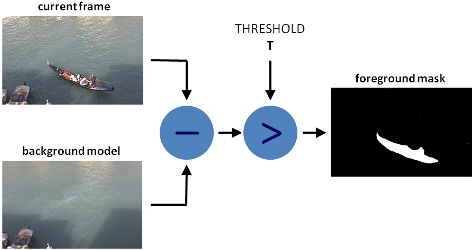
\includegraphics[scale=0.9]{D:/COMP30040/report/pic/2/Background_Subtraction_Tutorial_Scheme.png} 
  \caption{背景消除流程}
\end{figure}
从“subtraction"一词我们能很容易想到最直接也最字面意义的方法:对两张图片相应像素作差。理想条件下北京在整个录像片段中不会变化,因此只要我们将第一帧视作纯背景之后就能用之后每一帧减去第一帧得到当前帧前景。由于背景不变,因此相应帧像素作差为0,而前景帧像素与背景帧相应像素作差结果非0,再通过将该差值图二值化便可区分前景和背景。\\
但完全静态背景基本无法实现,或者说背景时刻会有微小变化。这需要我们实时更新背景,否则变化后的背景会被误分类为前景,在最终的二值图中成为噪点并对我们区分前景造成困难。\\
一种更新背景的方法是利用由Friedman和Russell提出的高斯混合模型 [8]。在该方法中,我们假设不管背景色彩如何变化都会落在能表示背景模型的一系列高斯簇中。我们尝试对每个像素做二分类来决定其属于背景或是前景。\\
给定一段视频,第一帧会被假设为背景帧并用于建立高斯混合模型。对于后续每一帧,其每个像素会被二分类,得到的背景被用于更新模型,该新模型则被用于对下一帧作减法。通过该方式可实现背景的实时更新,早于一定时间的历史信息则被丢掉。\\
在运动员检测中,运动员应被当作前景。由于他们在时刻运动从而与几乎静止的背景有显著区别,因此可被较容易的区分出来。然而需要注意的是足球也在运动,因此还需采取其他措施在二值图中过滤掉其相应连通区域。
\subsubsection{用基于 HOG 的 SVM 进行检测}
特征描述子是一些从图片中提取出的,有一定实际意义且能一定程度表示图片的数据。在众多种类的描述子中,Dalal 和 Triggs [9] 提出的 HOG 特征被广泛运用于人像识别。
\begin{figure}
  \centering
  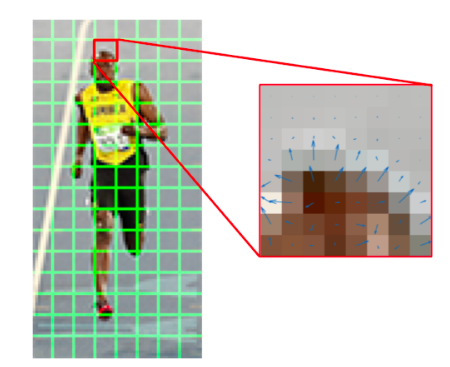
\includegraphics[scale=0.5]{D:/COMP30040/report/pic/2/Sample_of_gradients.png}
  \caption{A heuristic view of gradients in a cell}
\end{figure}
\begin{figure}
  \centering
  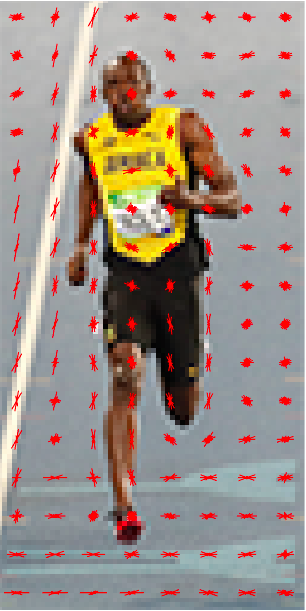
\includegraphics[scale=0.3]{D:/COMP30040/report/pic/2/HOG_of_a_picture.png} 
  \caption{某个检测窗内的HOG。}
\end{figure}
对每个从原始图片划分出的胞元,我们在其中计算图像梯度。一组相邻胞元组成区块,一个区块内的所有方向梯度依照其方向被分入不同筐并组成该区块的HOG,而所有区块的 HOG 连接起来最终组合成整张图片的 HOG 。这之后,我们可以在训练集上根据 HOG 特征训练一 SVM 分类器,如同 [9] 所做。在检测环节,我们用一个扫描窗扫过整张图片,并在每一步对扫描窗内图像用 SVM 进行分类以确定其是否包含运动员人像。

\subsubsection{用 Mask-RCNN 检测}
CNN会从图片中隐式而非显式提取信息。由于CNN网络可让我们十分方便的为模型增加非线性,其对于检测,分割与分类人物有格外出众的效果并且已经成为处理图片相关任务的首选。\\
\begin{figure}
  \centering
  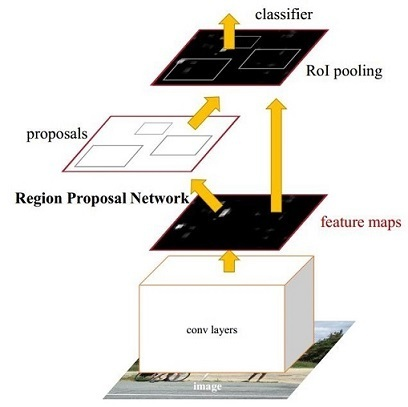
\includegraphics[scale=0.5]{D:/COMP30040/report/pic/2/RCNN_arch.jpg} 
  \caption{Architecture of Faster-RCNN}
\end{figure}
经过若干年的发展,CNN 获得了更强的进行实例分割的能力。当前最前沿技术为 Mask-RCNN. 其中结构类似 Faster-RCNN 的部分被用于目标检测,而类似 FCN 的部分则被用于分割。在本项目中我们只用到检测部分,因此将重点聚焦 Faster-RCNN 子结构。\\
不同于低效的窗扫描方法,在 Faster-RCNN 中预训练的 RPN 被用于在特征图上生成可能的检测框。\\
\begin{figure}
  \centering
  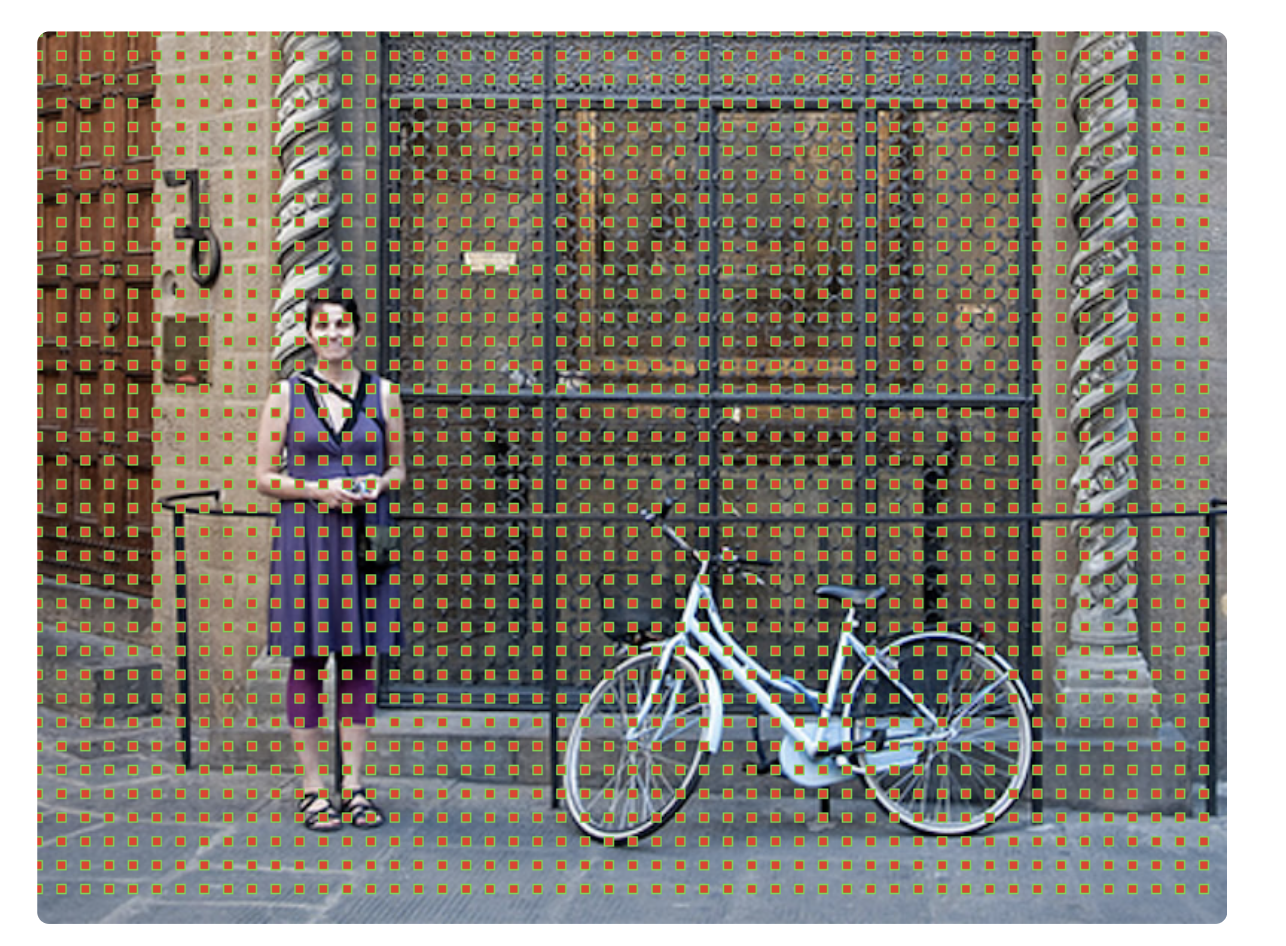
\includegraphics[scale=0.25]{D:/COMP30040/report/pic/2/anchor_point.png} 
  \caption{原始图像上的锚点示例。}
\end{figure}
在RPN中, 每个特征图上的点在原图中相应位置被当作锚点,基于每个锚点生成9个大小尺寸不同的候选检测框并判定其中是否有物体。不含物体的检测框被抹消,而含有物体的则通过边框回归调整其大小及位置以使得其尽量贴合物体外轮廓。判定生成检测框与给定检测框间相似程度的函数被包含进了损失函数并在训练阶段进行梯度下降,因此在使用阶段边框回归可自动完成。再得到的若干检测框将用非极大值抑制处理以舍弃 IoU 值高者。\\
RPN输出的检测框被用于在池化层中从特征图上抽取特征,之后使用若干全接层进行一维化。全接层的输出会被分别放入两个分支,第一个用于给出分类结果,第二个用于进一步进行边框回归。与RPN中的边框回归不同的是,在RPN中所有检测框按统一方式回归,而此处根据每个检测框分类结果不同会有相应不同的回归方式。\\
最终输出为标有检测框的图片,且每个检测框配有相应分类结果。
\subsection{分类}
在获取当前帧的监测结果后,识别出的运动员仍需要被分类以标明身分并在追踪中正确更新信息。在录播中,人脸检测由于低清晰度和运动时的进一步模糊而无法实现,所以应选择更加明显且不随尺度及旋转改变的特征。
\subsubsection{特征}
\paragraph{4.3.1.1 RGB 直方图}
人类可通过衣服的颜色对不同的人进行区分,计算机或许也可在分类工作中利用颜色信息。采用原始颜色信息可能不甚明智,因为这会使向量中包含相似特征--例如稍浅的蓝色与稍深的蓝色。相近特征不会对表示图片有益而徒增计算量,因此我们采用RGB直方图。对每个颜色通道,某个值内的颜色将被统一放到一个框中,每个直方图代表各范围的颜色在图中出现的频率。将三通道的直方图拼起来后可作为分类用的特征向量。
\paragraph{2.3.1.2 SIFT 描述子}
运动员总在持续移动。他们远离摄像机时会在屏幕中显得更小,而靠近摄像机时则变得更大;他们面向的方向时刻变化并且姿态时刻不同。尽管以上种种,我们还是像将某个“运动员A”正确分类为“运动员A”,不管他在屏幕里是什么样子,所以我们需要不随尺寸变化或旋转发生改变,或改变较小的特征。Lowe 提出的 SIFT [11] 满足上述要求。提取该特征分为以下四步:
\begin{figure}
  \centering
  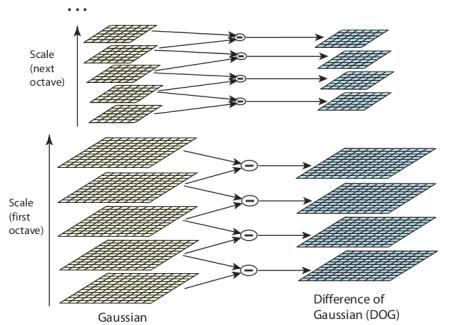
\includegraphics[scale=0.5]{D:/COMP30040/report/pic/2/sift_dog.jpg} 
  \caption{Doing DoG on adjacent $\delta$ s.}
\end{figure}
\begin{figure}
  \centering
  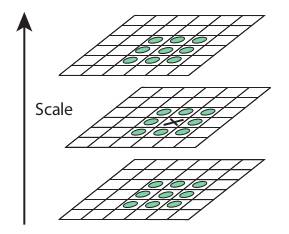
\includegraphics[scale=0.5]{D:/COMP30040/report/pic/2/sift_local_extrema.jpg} 
  \caption{寻找区域极值。}
\end{figure}
\begin{itemize}
\item 1. 尺度空间极大值检测: 高斯差算法被用于高效搜索图片并寻找潜在关键点。高斯模糊滤波器在一系列不同尺度中被使用,通过计算相邻尺度图片的差可得到差分图。我们通过将每个像素与同尺度空间内相邻8个像素与相邻尺度空间内的9像素作比较寻找区域极小与极大值并将其视为潜在的关键点。
\item 2. 关键点本地化:首先在候选关键点选出在不同尺度与旋转下保持不变的那些。边缘相应与低对比度关键点将被移除。我们通过利用相邻尺度的信息寻找最合适的尺度从而优化位置。
\item 3. 方向指派:对每个关键点的相邻区域,我们计算其 HOG,用36个框表示360度。频率最高的框将被选为主方向并用其正则化整个向量,此后所有计算将基于此方向。
\item 4. 关键点描述子:关键点周围的区域将被分为16个胞元(每个子区域4个),并在每个胞元上计算8个框的 HOG。 这些 HOG 将被拼接为长128的特征向量来表示该区域。
\end{itemize}
\paragraph{2.1.3.3 MSER}
最大极值稳定区域(MSER)是那些在不同阈值下保持面积恒定的连通区域。直观而言,这些区域的颜色将与周围显著不同,因此可被当作感兴趣区域。在 [3] 中,SIFT从检测框的MSER中被计算出。
\subsubsection{视觉词包}
\begin{figure}
  \centering
  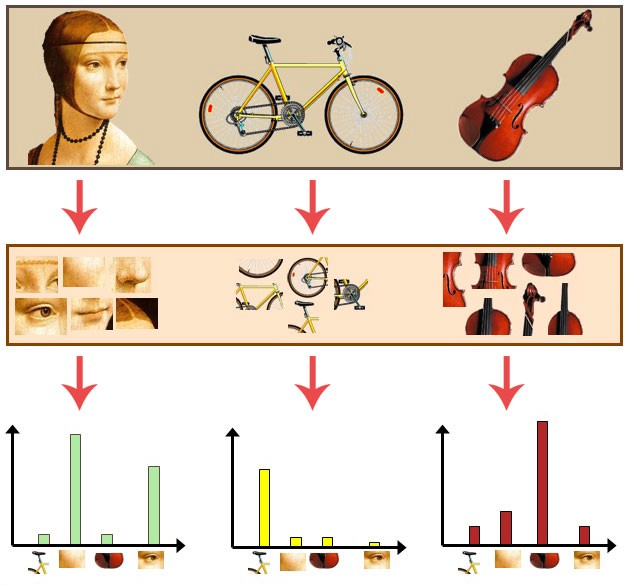
\includegraphics[scale=0.4]{D:/COMP30040/report/pic/2/build_BOVW_histogram.jpeg} 
  \caption{建立视觉词包直方图}
\end{figure}
视觉词包(BOVW)模型来源于NLP领域,其尝试用一系列视觉词表示图片。在 [3] 中,来自 MSER 的 SIFT不被直接用于分类,而是首先被分类到不同的视觉词下,再用视觉词直方图作为图片的特征向量。如此操作原因有二:
\begin{itemize}
\item 1. 从不同图片中提取的 SIFT 数量不同。众所周知,放入分类器的特征向量需要具有相同的长度,因此这些原始 SIFT 特征需要以某种方式进行长度统一。
\item 2. 在一张图片中,某些SIFT描述子可能代表了相同的,或至少相似的特征,此外,某图片中的一组 SIFT 特征还可能与另一图片中的另一组 SIFT 特征相似。若把它们不加区别的放进特征向量,则只会增加计算量。
\end{itemize}
\subsubsection{分类器}
在收集特征向量并退长度进行统一后他们便可被放入分类器。这里我使用KNN分类器。\\
训练分类器十分简单:只需将特征向量同其标签放到向量空间中。在分类时首先应选定超参数K,之后选择离测试样例向量最近的K个向量并将占多数的那个赋给测试样例。这里K不可过小,否则分类过程会轻易受到噪声扰动;也不可过大,否则增大极端负担的危害会超过减轻过拟合的好处,同时邻近类别边界的向量很可能会有来自若干类别的数量相等的相邻向量,为赋标签带来困难。
\subsection{追踪}
当我们在连续帧中收集检测结果时,我们还应将同一运动员的检测结果连接起来以给出轨迹信息。在该项目中,这将用 Tracking-by-detection 思想,通过将每个新检测结果赋给一个追踪片段实现。
\begin{figure}
  \centering
  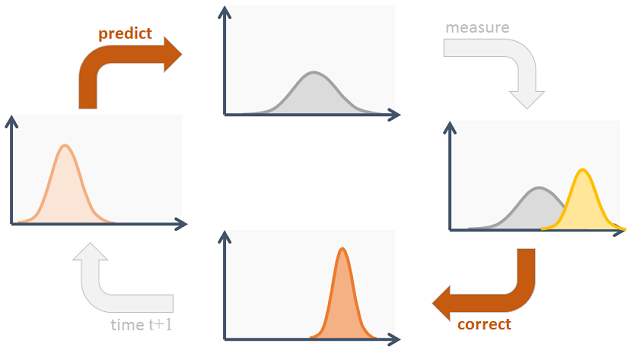
\includegraphics[scale=0.4]{D:/COMP30040/report/pic/2/kf_workflow.jpeg} 
  \caption{Kalman 滤波器工作流程直观表示}
\end{figure}
\subsubsection{Kalman 滤波器}
Kalman 滤波器 [12] 在考虑系统及背景噪音的基础上提供了一种综合使用观测值和预测值的方法。基于 Kalman filter 的状态估计将比完全依靠不精确的观测值更为准确。\\
在运动员追踪中,运动员位置是我们需要跟踪的信息,其历史信息按时序被保存在为其维护的追踪片段中。对每个运动员而言,其当前帧位置的预测首先在历史信息的基础上通过滤波器被给出,预测被建立在运动员在帧与帧之间移动轨迹近似线性的假设上,所以可给出滤波器的状态转移矩阵:\\
\begin{align*}
x_k = x_{k-1}+v_{k-1}^x \\
y_k = y_{k-1}+v_{k-1}^y
\end{align*}
where 
\begin{align*}
v_{k-1}^a = a_{k-1} - a_{k-2}, \: a=x \: \text{or} \:y
\end{align*}
在相应检测结果被找到之后,它会与给出的预测在滤波器中被组合并给出当前帧位置的最终结论,而对下一帧位置的预测又可被给出。在每一帧中我们重复此操作以更新运动员位置信息并将其存入追踪片段,如此实现追踪。
\subsubsection{时序连贯}
决定检测结果与追踪片段间匹配方式的方法不是简单的将某个检测结果与具有相同标签的预测进行匹配,因为分类结果也可能有误。此处采用的方法是基于时序连贯性。运动员的速度是有限的,因此其在相邻两帧之间移动的距离也应该是有限的。\\
根据该常识,我们可以将假设的运动员运动的最大可能距离定为超参数。在匹配所有追踪片段与新检测结果后,我们检查追踪片段给出的预测与匹配到的检测结果间的欧式距离是否小于该阈值。若合格,则将检测结果与匹配的预测结合给出最终结果,否则该检测结果会由于潜在的错误被追踪片段拒绝,而该追踪片段会仅用预测结果作为当前帧最终结果。
\newpage
\section{实现}
在该部分中我描述了在系统实现中尝试过的各种方法。
\subsection{系统工作流程}
在系统开始工作前,首先应准备好用于运动员检测和分类的模型。目标录像将被循环两遍。在第一次循环中,首先在每一帧中寻找检测结果,用分类器给出标签并赋给相应的追踪片段。在该循环结束后,只含错误检测结果的片段将被滤掉,标签检测在剩余片段上进行。这些片段会被根据第一个检测结果出现的时间从小到大排序,最终在第二遍循环中画到目标录播上。
\subsection{检测}
\subsubsection{先验知识}
一些先验知识被用于一定程度上筛去假阳并加速检测。\\
一个常识是在静止相机的录像中代表球场的区域始终不变,此外,运动员不能跑到球场之外。因此在每一帧中我们只对球场代表的区域进行检测,这可以通过扫描更小的区域来加速检测,也可以避免在运动员永远不可能出现的区域得到假阳。
\begin{figure}
  \centering
  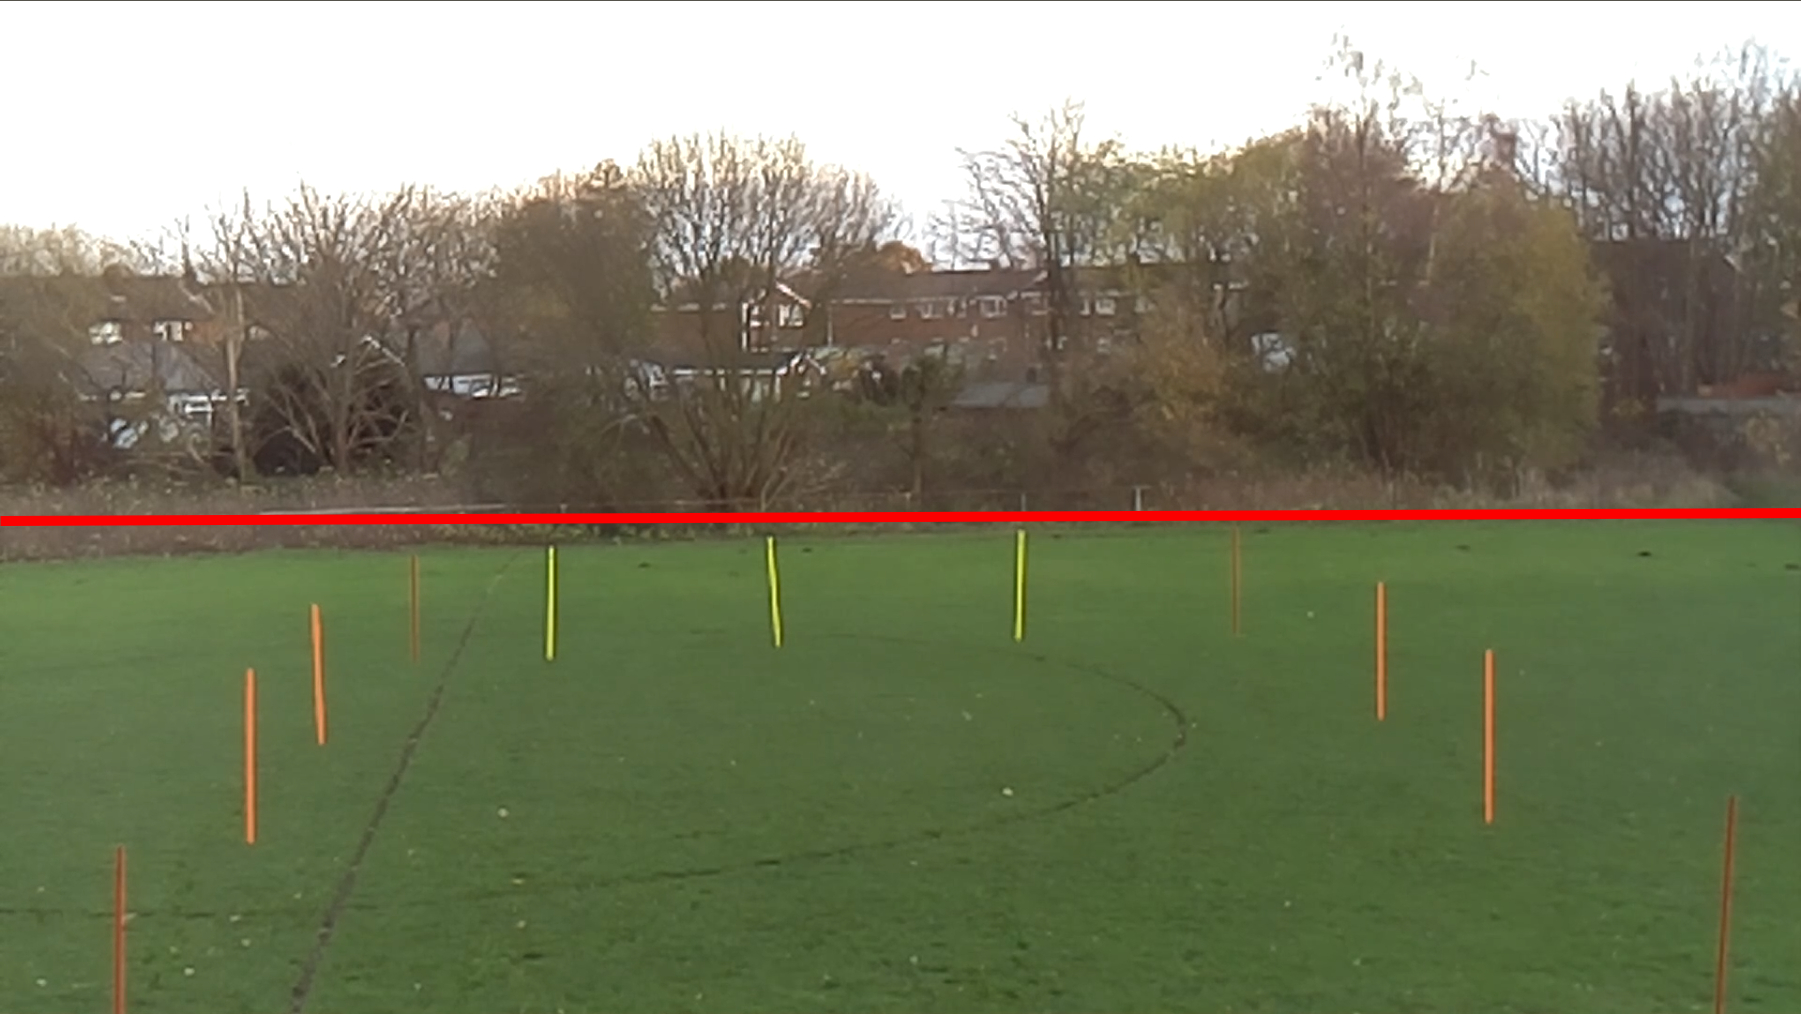
\includegraphics[scale=0.2]{D:/COMP30040/report/pic/3/background.jpg} 
  \caption{纯背景,只有红线下的区域会被检测}
\end{figure}
\begin{figure}
  \centering
  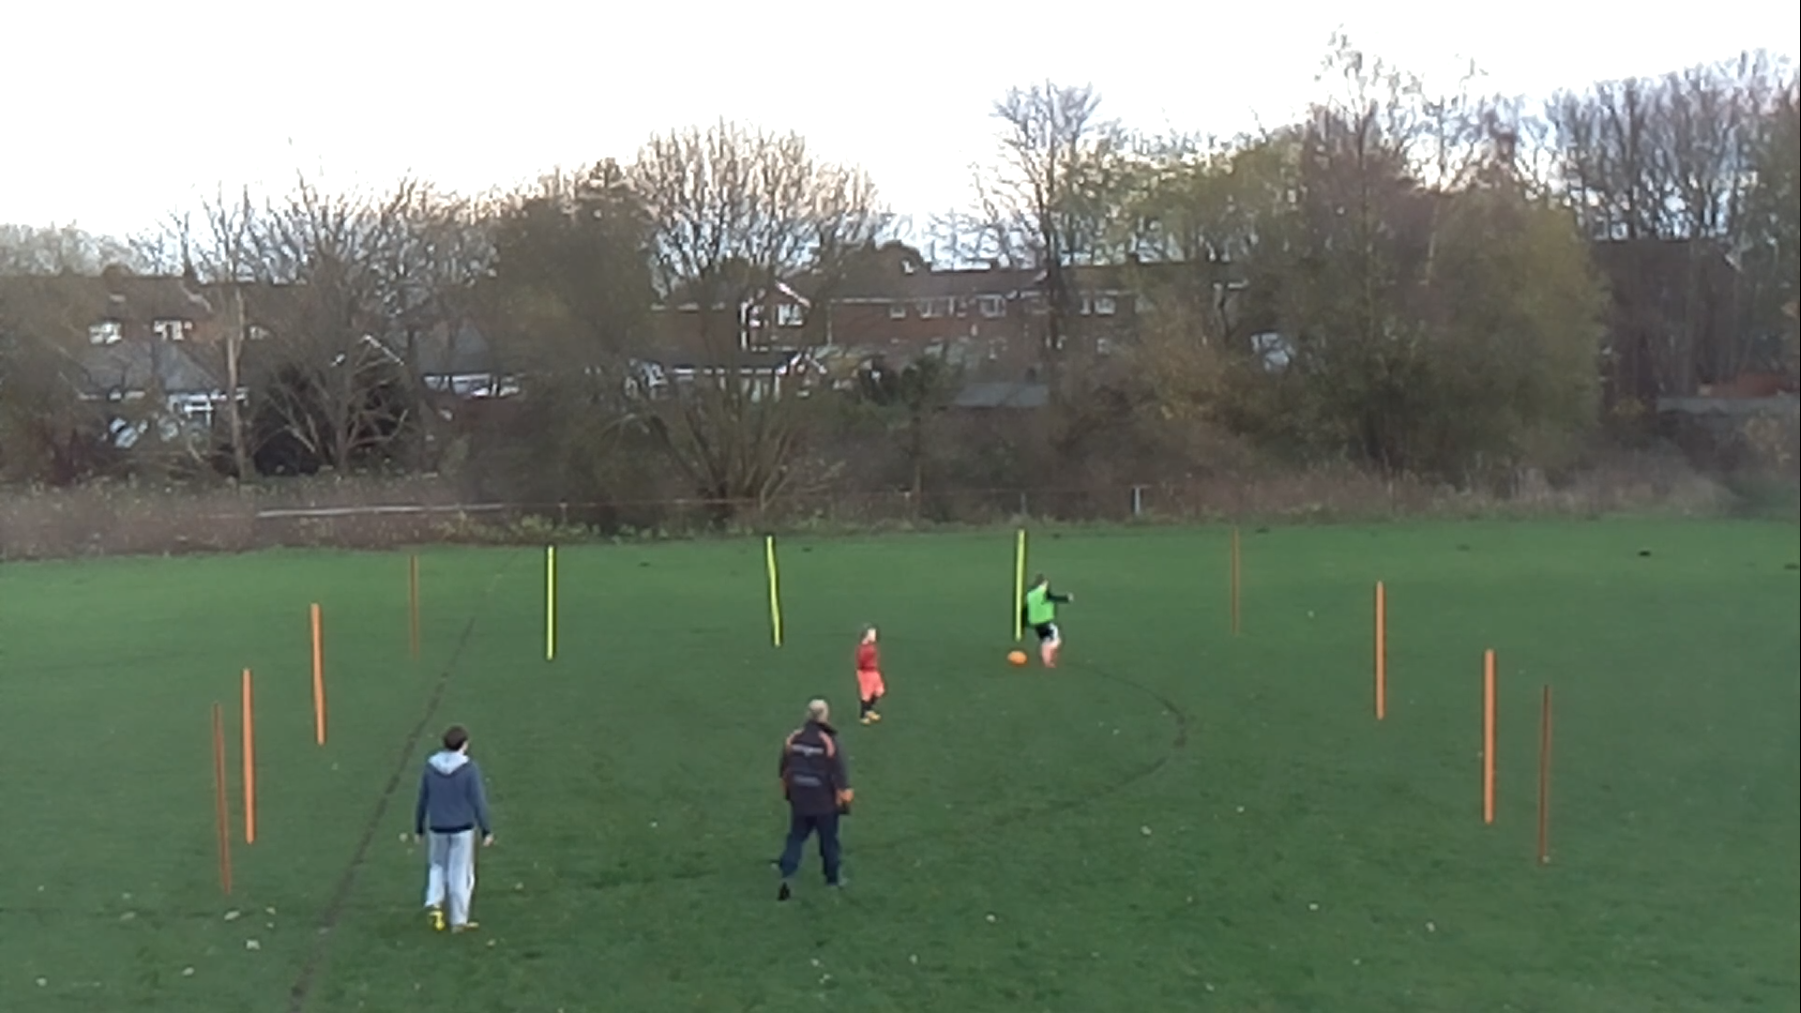
\includegraphics[scale=0.2]{D:/COMP30040/report/pic/3/foreground.png} 
  \caption{背景与运动员}
\end{figure}
此外,运动员的检测框不会过大或过小,过宽或过窄。尽管检测框的尺度可能随着运动员与相机的距离变化而变化,但仍应保持在一定范围内。因此不符合要求的检测框会被舍弃。
\subsubsection{Background subtraction}
起初我尝试用背景消除作为基准。对于静止相机给出的录像,背景基本不变,因此在一开始给出纯背景图并从之后每一帧减去该背景是可行的。\\
我采用的背景消除算法来自 OpenCV [13], 基于高斯混合模型实现。\\
我们可以从图  中看到在数据集中前景与背景很容易区分,因此我们也可猜想他们的像素值有明显不同,从直觉出发我们可以很容易地将背景帧从其余帧中减去,连通区域便代表了运动员的位置。一开始,背景模型会先从当前帧中被减去并用背景像素进行更新,差分图再用阈值过滤得到的阴影。过小的连通区域代表了足球和噪点,因此我们用一个阈值将其过滤掉。对剩下的连通区域,OpenCV 中的 findcontours 函数被用来根据连通区域轮廓中x,y坐标的最小及最大值画检测框。其优点是画出的长方形会紧贴运动员从而较为精确地表示运动员的位置,且在框中含有较少的无关信息。
一些检测结果示例在下图给出。
\begin{figure}[h!]
  \begin{subfigure}[b]{\linewidth}
  \centering
    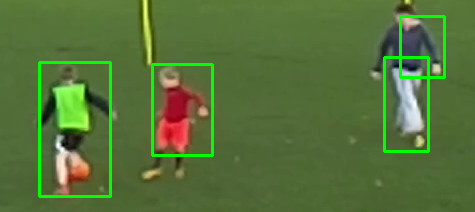
\includegraphics[scale=0.4]{D:/COMP30040/report/pic/3/multi_box_2.png} 
  \end{subfigure}
  \begin{subfigure}[b]{\linewidth}
  \centering
    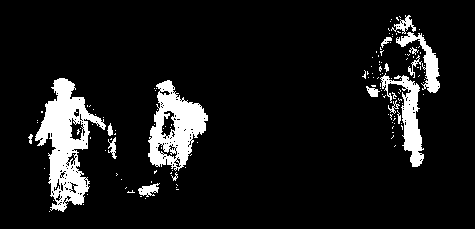
\includegraphics[scale=0.4]{D:/COMP30040/report/pic/3/multi_box_1.png} 
  \end{subfigure}
  \caption{有时由于连通区域不完整,检测框无法涵盖整个运动员}
\end{figure}
\begin{figure}[h!]
  \centering
  \begin{subfigure}[b]{0.4\linewidth}
    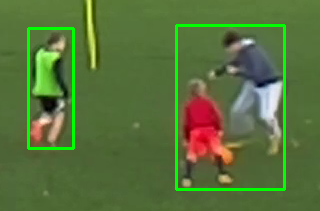
\includegraphics[scale=0.4]{D:/COMP30040/report/pic/3/occlusion_1.png} 
  \end{subfigure}
  \begin{subfigure}[b]{0.4\linewidth}
    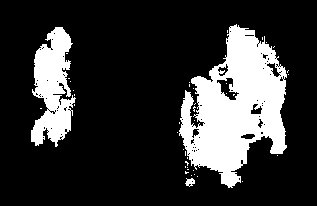
\includegraphics[scale=0.4]{D:/COMP30040/report/pic/3/occlusion_0.png} 
  \end{subfigure}
  \caption{背景消除无法区分球员}
\end{figure}
从图 的样例中我们可以看到背景消除有可能会严重阻碍后续步骤的一些缺点。\\
首先,其对遮挡过于脆弱。当遮挡发生时,在二值图中的相应位置我们只能知道“这里代表的东西和背景不一样”,但我们无法知道它代表了两个人,因为那里只有一个连通区域。能帮助我们判断“此处有两个人”的其它信息都在消除过程中被丢掉。其次,一个运动员相应的连通区域不总是互相连接,导致检测框不能包含整个人像。\\
我尝试了至少解决第二个问题,这通过若干次形态学膨胀与侵蚀以连接属于同一运动员的连通区域从而让每个运动员有正好一个尺寸正确的检测框实现。\\
\begin{figure}[h!]
  \begin{subfigure}[b]{\linewidth}
  \centering
    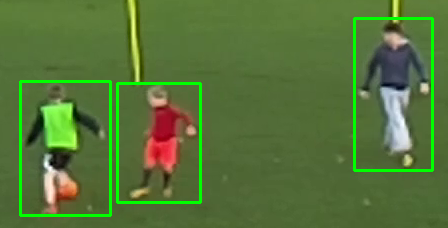
\includegraphics[scale=0.4]{D:/COMP30040/report/pic/3/complete_blob_1.png} 
  \end{subfigure}
  \begin{subfigure}[b]{\linewidth}
  \centering
    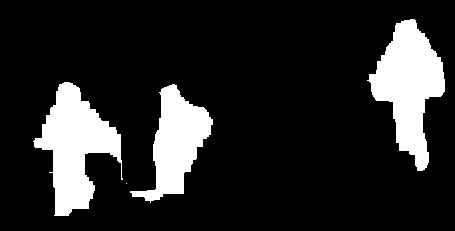
\includegraphics[scale=0.4]{D:/COMP30040/report/pic/3/complete_blob.png} 
  \end{subfigure}
  \caption{通过形态学膨胀填充连通区域,再通过侵蚀恢复区域原有大小}
\end{figure}
我们可以看到第二个问题被成功解决,但剩下的一个问题对于背景消除而言仍旧难以处理。
\subsubsection{基于 HOG 的 SVM 分类器}
之后我决定使用 SVM 分离器。再迁册前应首先准备好分类器。对于每一帧,一个扫描窗将扫过全图,扫描窗每走一步都将窗内部分放入分类器以判断其中是否包含人像。我尝试过 OpenCV 中给定的检测器 [15]与自己训练的另一个。
\paragraph{给定检测器}
该检测器在 INRIA 数据集上被训练,因此是泛用版本。联系人类轮廓总体相似的常识,而 HOG 主要检测轮廓,我猜想运动员与一般人的 HOG 特征也应该相似。因此泛用检测器在运动员检测中应该有可被接受的结果。\\
\begin{figure}[h!]
  \centering
  \begin{subfigure}[b]{0.4\linewidth}
    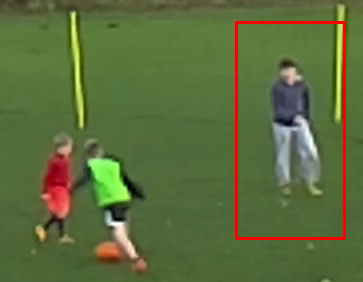
\includegraphics[scale=0.4]{D:/COMP30040/report/pic/3/vulnerability_to_occlusion_1.png} 
  \end{subfigure}\hspace{5mm}
  \begin{subfigure}[b]{0.4\linewidth}
    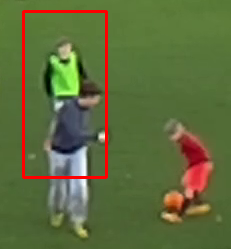
\includegraphics[scale=0.5]{D:/COMP30040/report/pic/3/vulnerbility_to_occlusion_2.png} 
  \end{subfigure}
  \caption{遮挡导致检测失败}
\end{figure}
然而其结果否认了我的猜想。我们可以看到泛用检测器给出了过多的假阴,因此不能给予足够数量的真阳以支撑连贯的追踪。其原因可能是 INRIA 数据集本身缺乏泛用性 -- 它只包含行人检测样本,但行人的 HOG 特征可能与互相相似但与运动员的 HOG 特征显著不同,因为运动员有更为多变的姿态。\\
\paragraph{自训练检测器}
之后我决定用给定的足球运动员数据集训练一个基于 HOG 的线性 SVM 检测器。 OpenCV 有计算 HOG 的函数 [16] 以及 SVM 检测器 [17],因此我只需提供训练样本。在加载训练样本后,每个训练样本会被在正中央剪裁出 64*128 的子图以符合 OpenCV 中对 SVM 扫描窗的内置要求。在子图上将被计算 HOG 特征并放入 SVM 进行训练。该轮训练结束后进行难例采集,得到的真阴将再次被放入 SVM 训练以提升其性能。对该 SVM 的使用应和对给定 SVM 的使用方法相同,只是这里要加载自己训练出的 SVM 。\\
一开始,我没有意识到可以只扫描图 中红线下方的版本并且只用了给定的数据集训练,但得到的分类器有很多错误。
\begin{figure}[h!]
  \begin{subfigure}[b]{\linewidth}
  \centering
    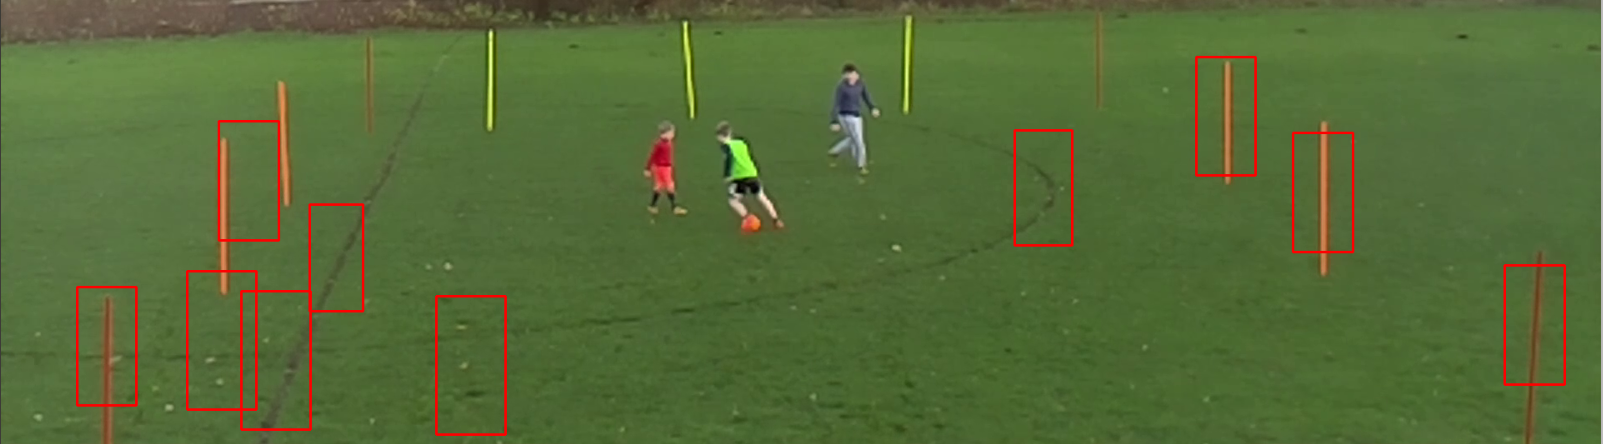
\includegraphics[scale=0.2]{D:/COMP30040/report/pic/3/selfHOG_1stround_2.png} 
  \end{subfigure}
  \begin{subfigure}[b]{\linewidth}
  \centering
    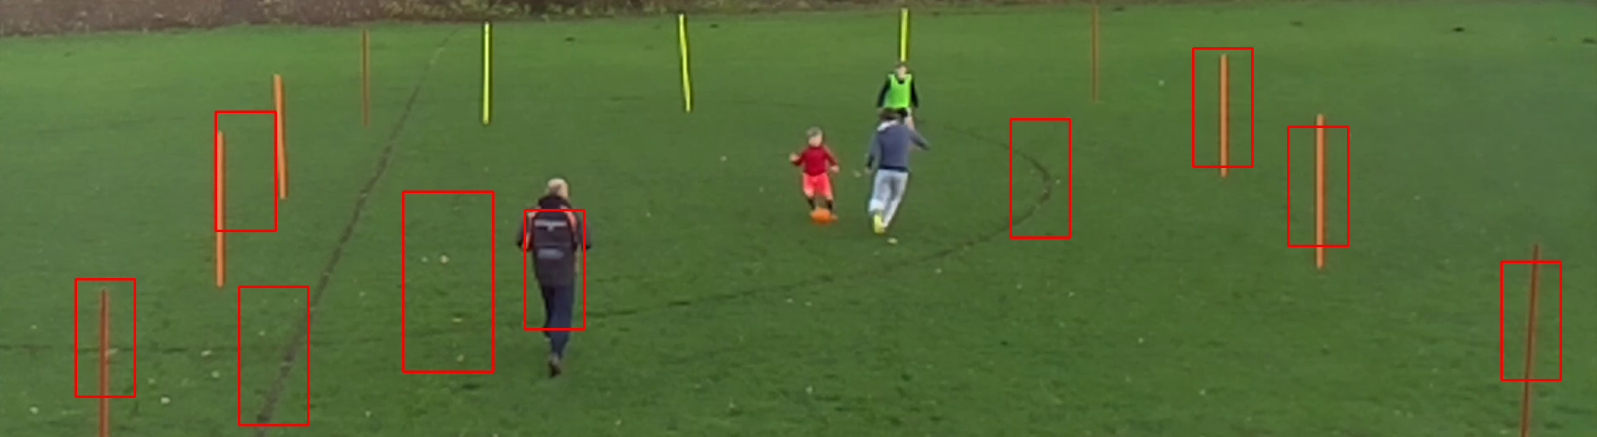
\includegraphics[scale=0.2]{D:/COMP30040/report/pic/3/selfHOG_1stround_1.png} 
  \end{subfigure}
  \caption{假阳过多,真阳过少}
\end{figure}

\begin{figure}[h!]
  \begin{subfigure}[b]{\linewidth}
  \centering
    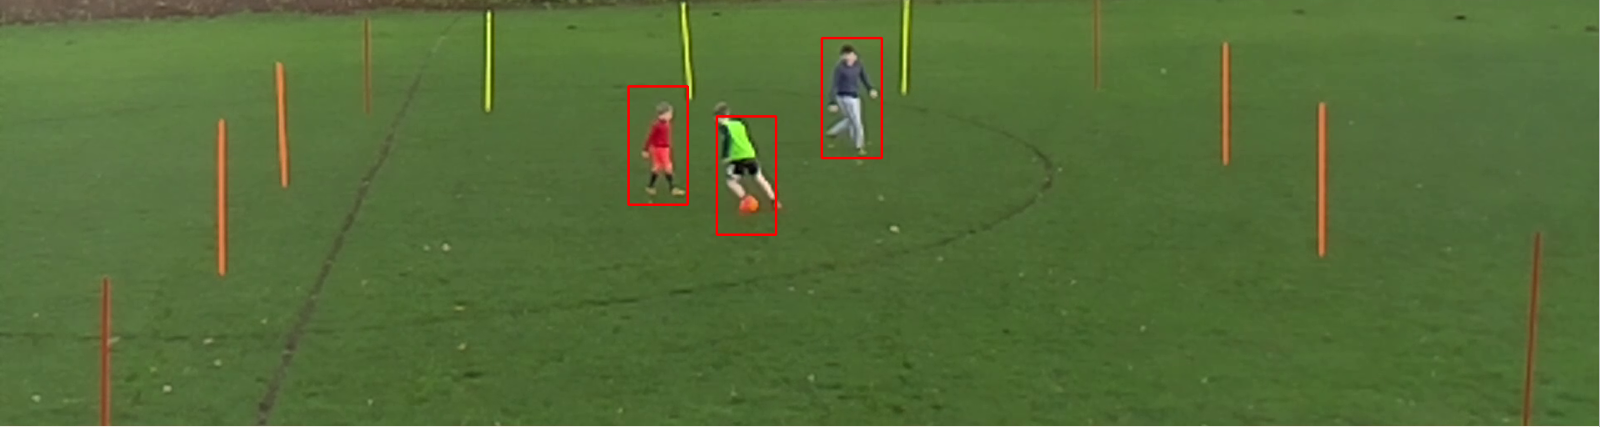
\includegraphics[scale=0.2]{D:/COMP30040/report/pic/3/selfHOG_2ndround_1.png} 
  \end{subfigure}
  \begin{subfigure}[b]{\linewidth}
  \centering
    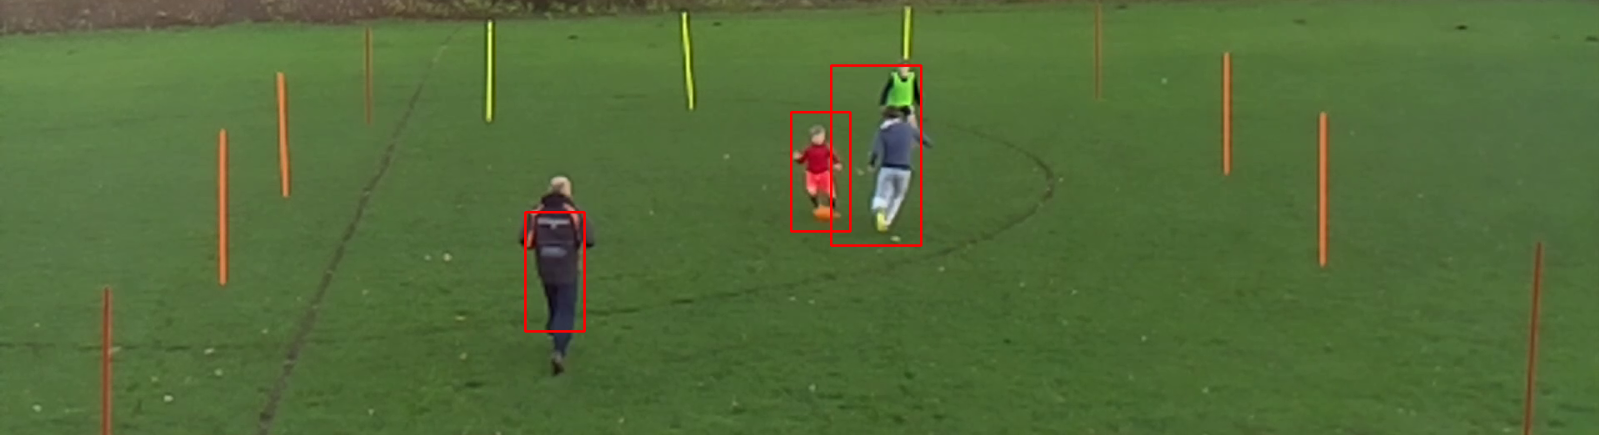
\includegraphics[scale=0.2]{D:/COMP30040/report/pic/3/selfHOG_2ndround_2.png} 
  \end{subfigure}
  \begin{subfigure}[b]{\linewidth}
  \centering
    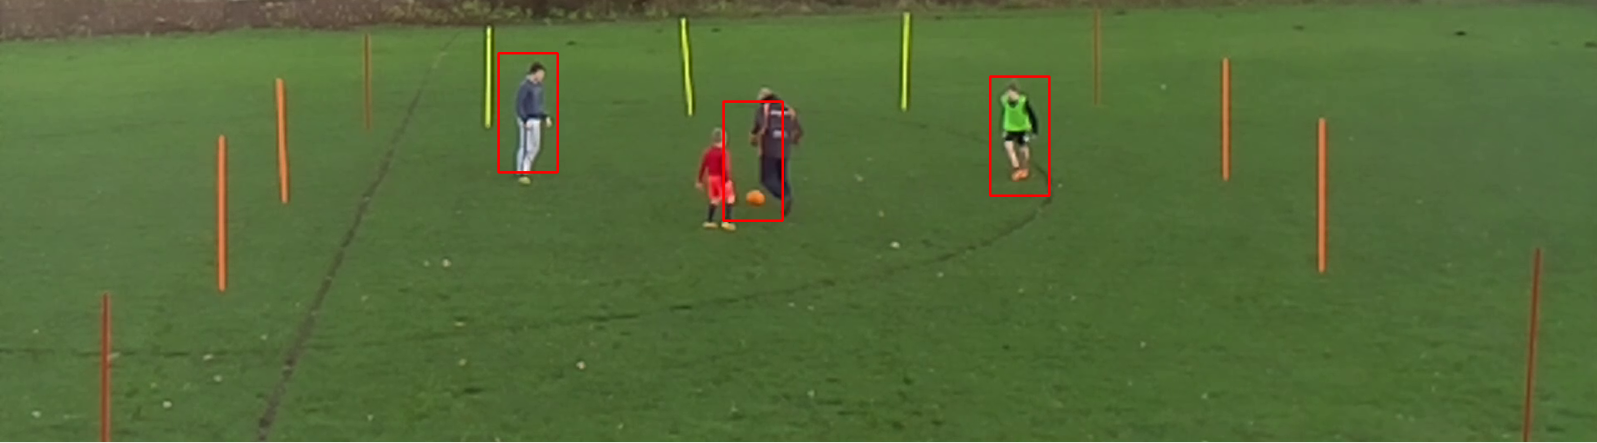
\includegraphics[scale=0.2]{D:/COMP30040/report/pic/3/selfHOG_2ndround_3.png} 
  \end{subfigure}
  \begin{subfigure}[b]{\linewidth}
  \centering
    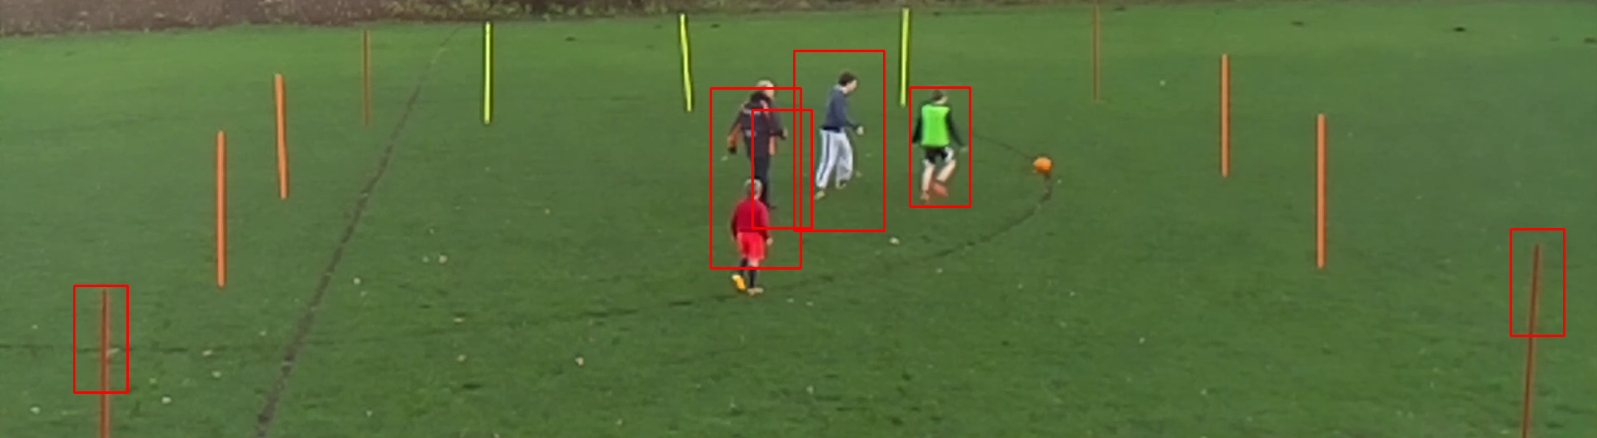
\includegraphics[scale=0.2]{D:/COMP30040/report/pic/3/selfHOG_2ndround_4.png} 
  \end{subfigure}
  \caption{假阳基本消除,但无法处理遮挡问题}
\end{figure}

\begin{figure}[h!]
  \begin{subfigure}[b]{\linewidth}
  \centering
    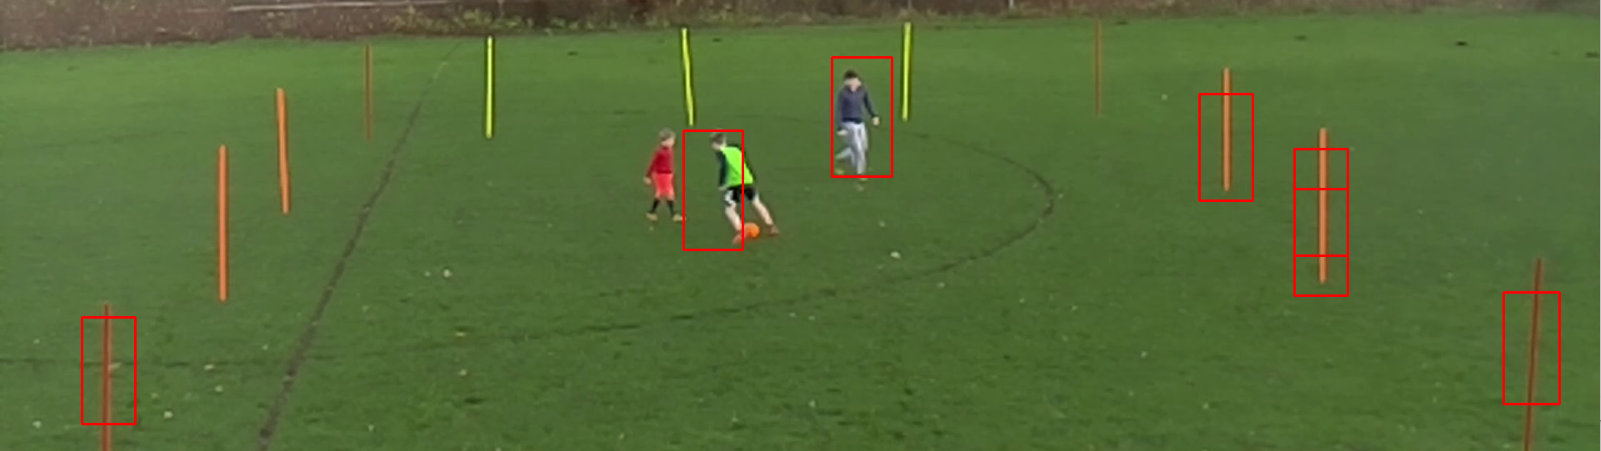
\includegraphics[scale=0.2]{D:/COMP30040/report/pic/3/selfHOG_3rdround_1.png} 
  \end{subfigure}
  \begin{subfigure}[b]{\linewidth}
  \centering
    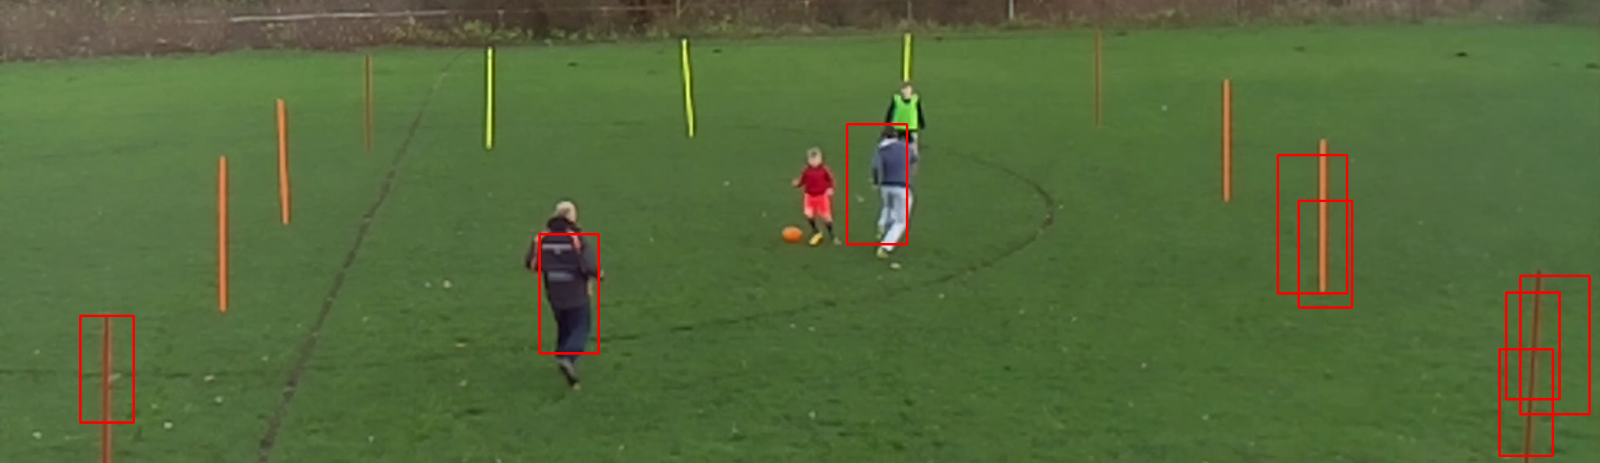
\includegraphics[scale=0.2]{D:/COMP30040/report/pic/3/selfHOG_3rdround_2.png} 
  \end{subfigure}
  \begin{subfigure}[b]{\linewidth}
  \centering
    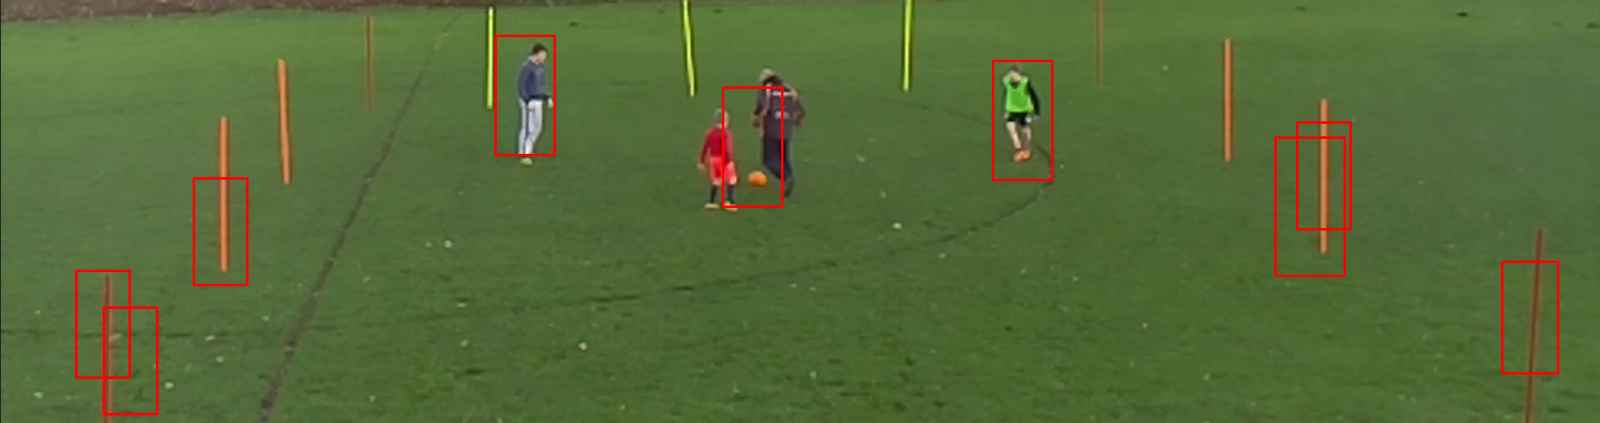
\includegraphics[scale=0.2]{D:/COMP30040/report/pic/3/selfHOG_3rdround_3.png} 
  \end{subfigure}
  \begin{subfigure}[b]{\linewidth}
  \centering
    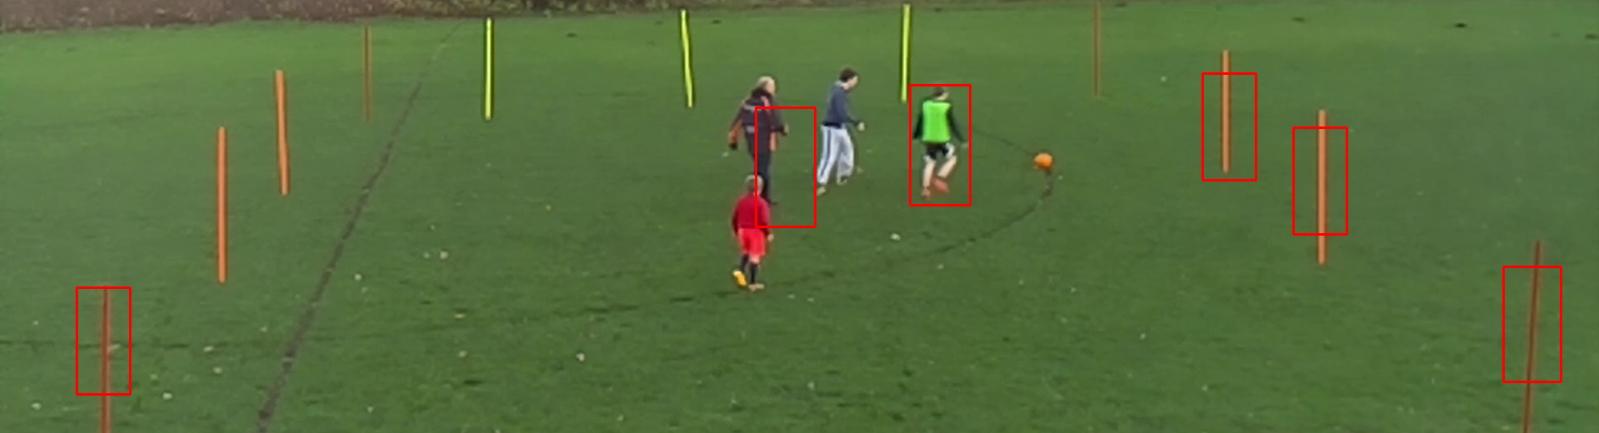
\includegraphics[scale=0.2]{D:/COMP30040/report/pic/3/selfHOG_3rdround_4.png} 
  \end{subfigure}
  \caption{遮挡问题未解决,但假阳重新出现}
\end{figure}

\begin{figure}[h!]
  \begin{subfigure}[b]{\linewidth}
  \centering
    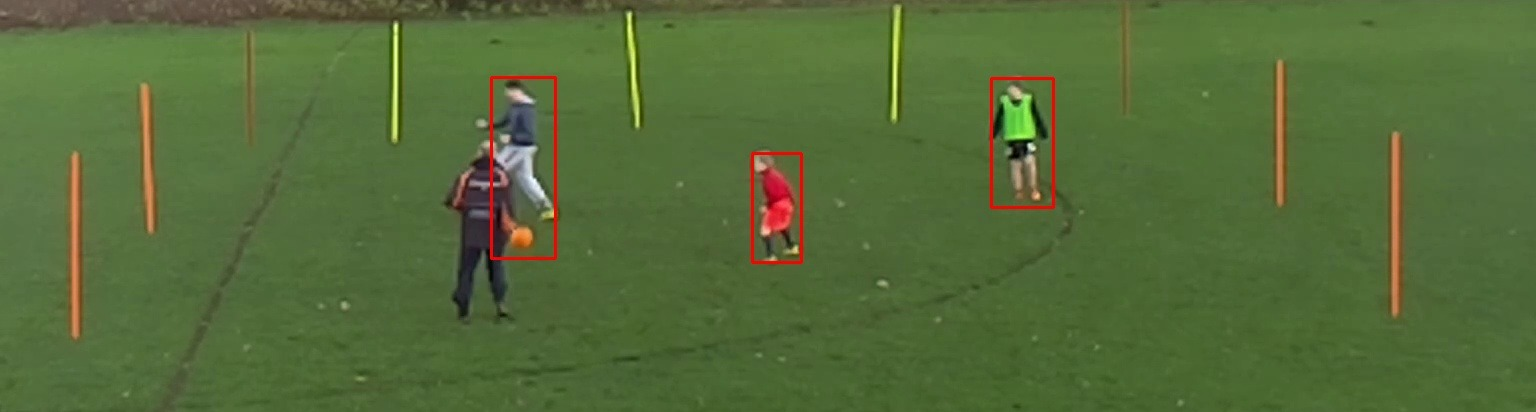
\includegraphics[scale=0.2]{D:/COMP30040/report/pic/3_new/det_occlu.jpg}
    \caption{轻度遮挡下的检测成功}
  \end{subfigure}
  \begin{subfigure}[b]{\linewidth}
  \centering
    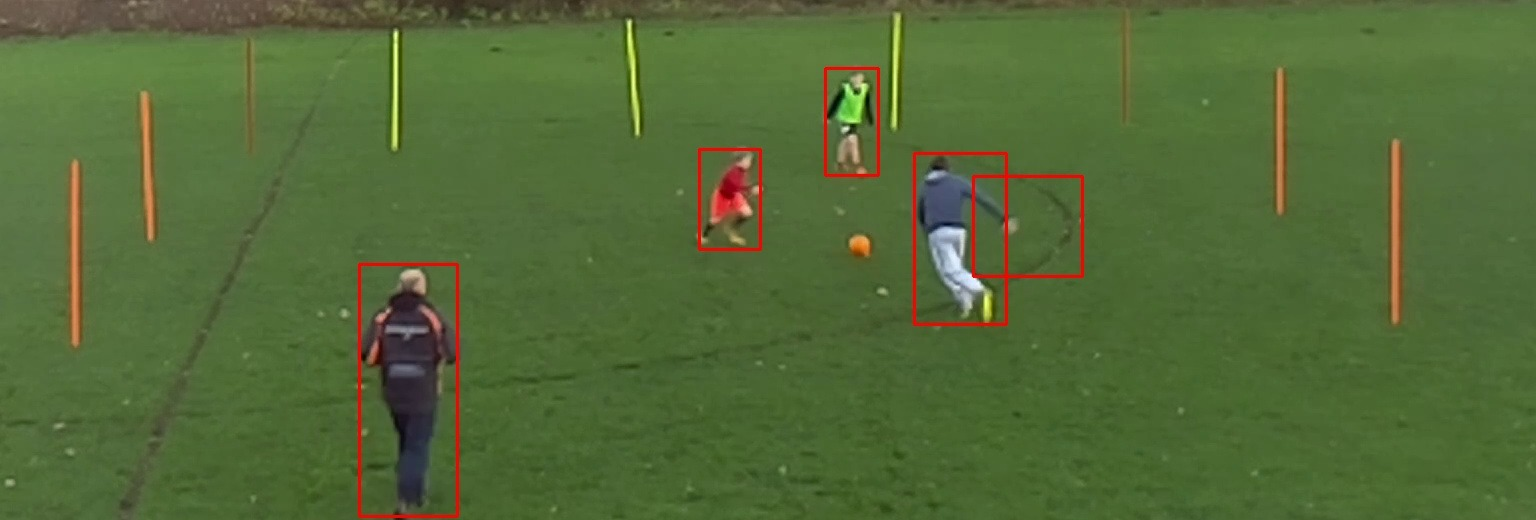
\includegraphics[scale=0.2]{D:/COMP30040/report/pic/3_new/false_posi.jpg} 
    \caption{假阳}
  \end{subfigure}
  \begin{subfigure}[b]{\linewidth}
  \centering
    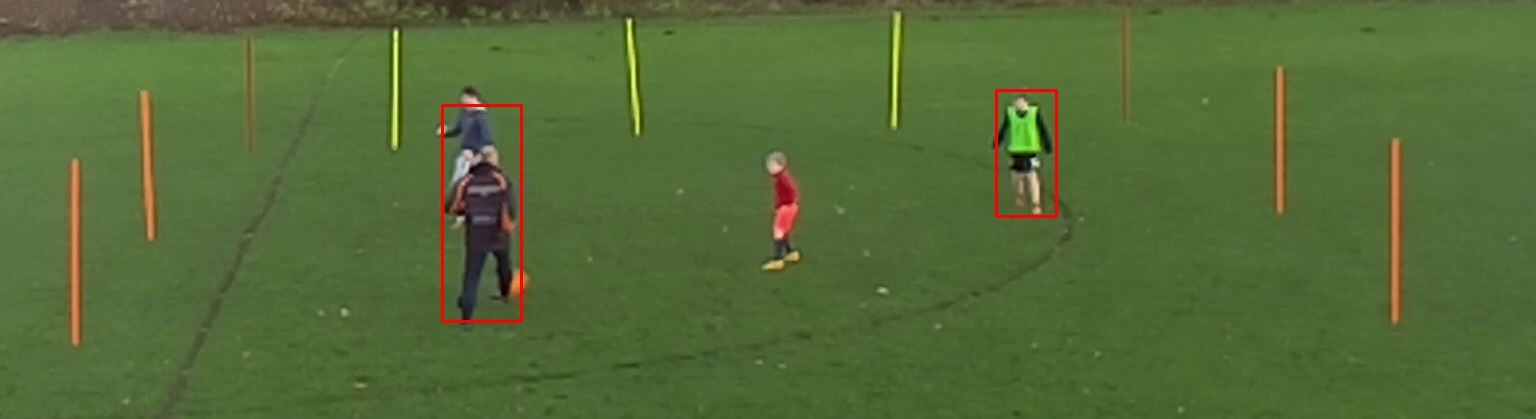
\includegraphics[scale=0.2]{D:/COMP30040/report/pic/3_new/failure.jpg} 
    \caption{严重遮挡下与对其他运动员的检测失败}
  \end{subfigure}
  \caption{Mask-RCNN 检测结果示例}
\end{figure}

从()结果可看出假阳过多而真阳过少,因此我把该轮所有检测输出至文件并分别增加了正负样本的数量。我如此操作了若干轮直到假阳基本消失。\\
从()结果可看出此时检测器能给出更为连续的检测,但另一问题仍旧存在:检测器在运动员仅仅距离相近但尚未发生遮挡的情况下检测便开始失败。我的猜想是描述遮挡的正样本过少,因此继续向训练集添加了对应的样本。\\
然而遮挡问题尚未解决,假阳却再次出现。鉴于在大样本上训练 SVM 并不明智,继续添加假阴样本并不是个好主意。我的猜想是在上一步添加正样本后 SVM 超平面无法再(基本)将所有正样本分到超平面一侧且更多的负样本被分到了正样本一侧。这可能是由于超平面缺乏非线性导致的。
\subsubsection{Mask-RCNN 检测器}
说到在模型中增加非线性,这是神经网络的专长。此外,相比 SVM 中 核技巧种类的限制,神经网络可以给出远远复杂的超平面。我采用的 Mask-RCNN 的实现来自于 [18] 并在之上做了少量修改以适应最新版本的 Keras 。\\
该模型在 MS COCO [19] 数据集上进行训练,包含91类物体的图片且其中涵盖人类。在神经网络中,卷积层会提取更隐性也更为全面的特征而非仅仅提取一类。\\
运动员检测工作可被当作神经网络的测试部分。当我们喂入一张图片,输出为图片的实例分割结果,其中每个物体包含一个上色的掩膜,一个标签及检测框。在该项目中我们只利用生成的检测框。
\paragraph{针对遮挡的先验知识}
不管该模型面对轻度遮挡效果有多么好,它在遮挡变严重时仍会失效。此处提出另一种先验知识以便在一定程度上减轻该问题。\\
通常情况下,在相邻两帧之间同一运动员的检测框大小不可突变,然而在遮挡发生时某个运动员的检测框会消失,而另一运动员的则会突然变大以包含两人。所以当上述情况发生,在上一帧中两个检测框的距离在一定阈值内,且当前帧中大小突变的检测框增大超过一定倍数阈值时,我们可知道此时发生了遮挡,且突然增大的那个检测框会被分解为两个更小的,其位置取决于两个运动员对应追踪片段给出的其当前位置的预测。\\
依据图 ,分解检测框有两种方式:若两个运动员从左上角及右下角相互靠近(通过遮挡还未发生时的上一帧的位置信息进行判断),则当前帧突然增大的检测框会被基于其左上角及右下角分解,新生成的两个小检测框具有和前一帧表示相应运动员的检测框相同大小;若两个运动员从左下角及右上角相互靠近,则检测框会被基于左下角及右上角分解。
\begin{figure}[h!]
  \begin{subfigure}[b]{\linewidth}
  \centering
    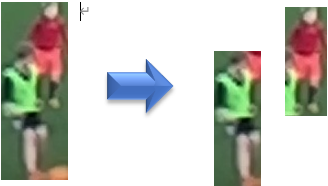
\includegraphics[scale=0.5]{D:/COMP30040/report/pic/3/heuristic_1.PNG} 
    \caption{基于左上角及右下角分解}
  \end{subfigure}
  \begin{subfigure}[b]{\linewidth}
  \centering
    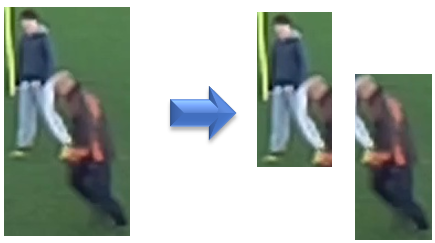
\includegraphics[scale=0.5]{D:/COMP30040/report/pic/3/heuristic_2.PNG} 
    \caption{基于左下角及右上角分解}
  \end{subfigure}
  \caption{}
\end{figure}

\begin{figure}[h!]
  \begin{subfigure}[b]{0.5\linewidth}
  \centering
	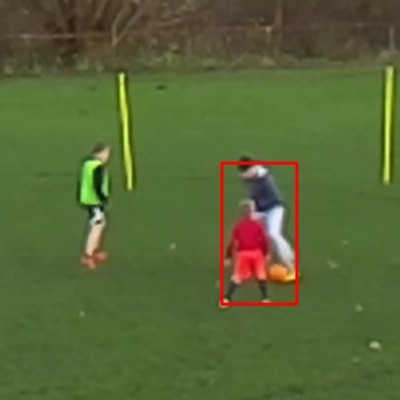
\includegraphics[scale=0.4]{D:/COMP30040/report/pic/3_new/off_1.jpg} 
  \end{subfigure}
  \begin{subfigure}[b]{0.5\linewidth}
  \centering
	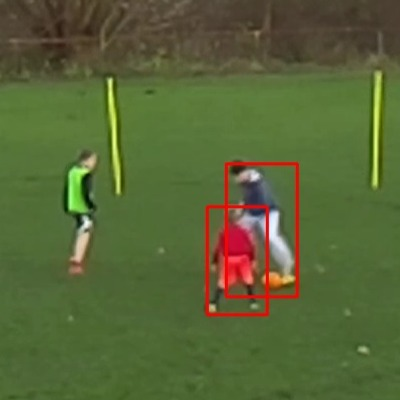
\includegraphics[scale=0.4]{D:/COMP30040/report/pic/3_new/on_1.jpg} 
  \end{subfigure}
  \begin{subfigure}[b]{0.5\linewidth}
  \centering
	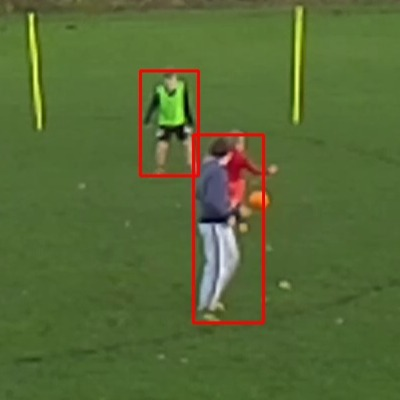
\includegraphics[scale=0.4]{D:/COMP30040/report/pic/3_new/off_2.jpg} 
  \end{subfigure}
  \begin{subfigure}[b]{0.5\linewidth}
  \centering
	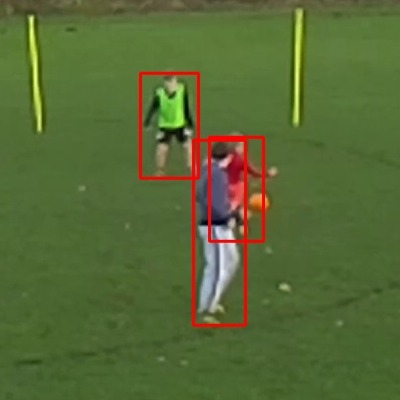
\includegraphics[scale=0.4]{D:/COMP30040/report/pic/3_new/on_2.jpg} 
  \end{subfigure}
  \begin{subfigure}[b]{0.5\linewidth}
  \centering
	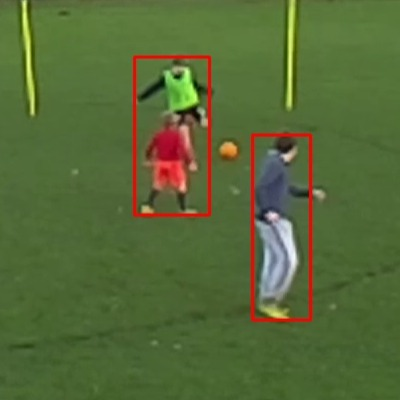
\includegraphics[scale=0.4]{D:/COMP30040/report/pic/3_new/off_3.jpg} 
  \end{subfigure}
  \begin{subfigure}[b]{0.5\linewidth}
  \centering
	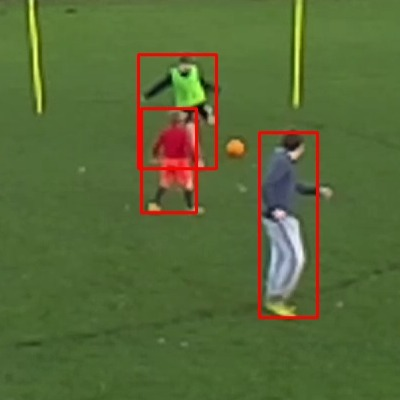
\includegraphics[scale=0.4]{D:/COMP30040/report/pic/3_new/on_3.jpg} 
  \end{subfigure}
  \caption{检测结果比较。左侧:未使用先验知识;右侧:使用先验知识}
\end{figure}

\begin{figure}[h!]
  \begin{subfigure}[b]{0.5\linewidth}
  \centering
	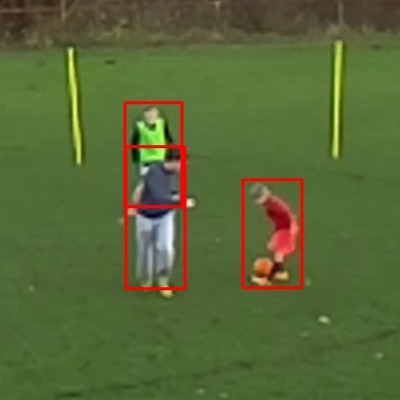
\includegraphics[scale=0.4]{D:/COMP30040/report/pic/3_new/off_seq_1.jpg} 
  \end{subfigure}
  \begin{subfigure}[b]{0.5\linewidth}
  \centering
	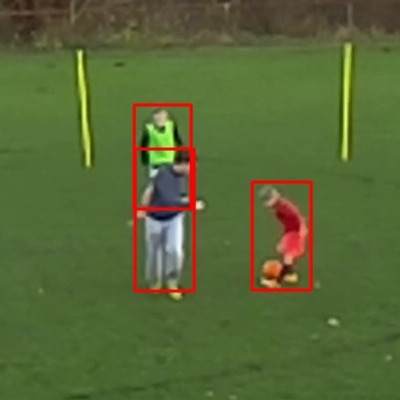
\includegraphics[scale=0.4]{D:/COMP30040/report/pic/3_new/on_seq_1.jpg} 
  \end{subfigure}
    \begin{subfigure}[b]{0.5\linewidth}
  \centering
	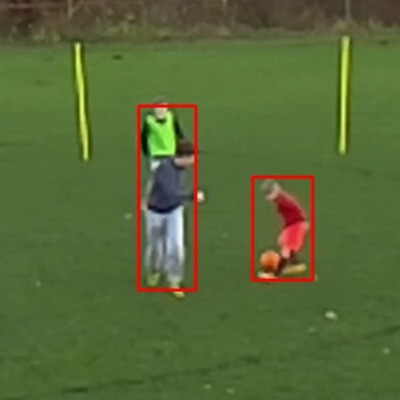
\includegraphics[scale=0.4]{D:/COMP30040/report/pic/3_new/off_seq_2.jpg} 
  \end{subfigure}
  \begin{subfigure}[b]{0.5\linewidth}
  \centering
	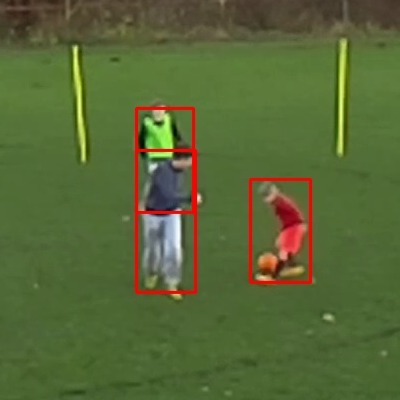
\includegraphics[scale=0.4]{D:/COMP30040/report/pic/3_new/on_seq_2.jpg} 
  \end{subfigure}
    \begin{subfigure}[b]{0.5\linewidth}
  \centering
	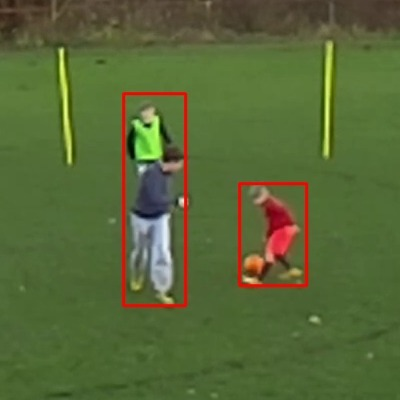
\includegraphics[scale=0.4]{D:/COMP30040/report/pic/3_new/off_seq_3.jpg} 
  \end{subfigure}
  \begin{subfigure}[b]{0.5\linewidth}
  \centering
	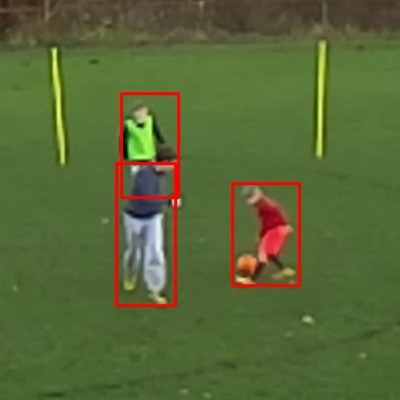
\includegraphics[scale=0.4]{D:/COMP30040/report/pic/3_new/on_seq_3.jpg} 
  \end{subfigure}
  \caption{时序检测结果比较(第一部分)。左侧:未使用先验知识;右侧:使用先验知识}
\end{figure}

\begin{figure}[h!]
  \begin{subfigure}[b]{0.5\linewidth}
  \centering
	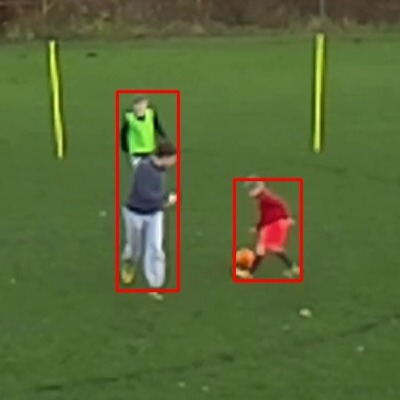
\includegraphics[scale=0.4]{D:/COMP30040/report/pic/3_new/off_seq_4.jpg} 
  \end{subfigure}
  \begin{subfigure}[b]{0.5\linewidth}
  \centering
	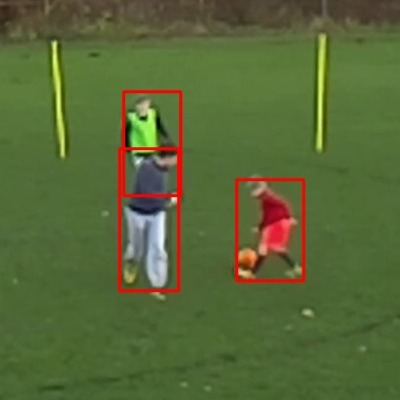
\includegraphics[scale=0.4]{D:/COMP30040/report/pic/3_new/on_seq_4.jpg} 
  \end{subfigure}
    \begin{subfigure}[b]{0.5\linewidth}
  \centering
	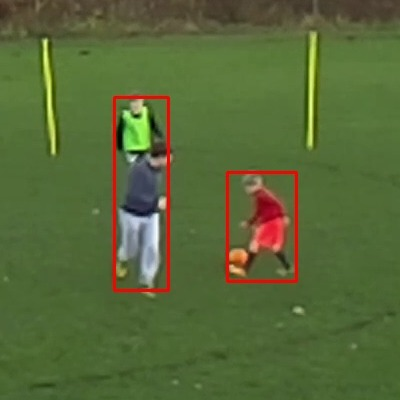
\includegraphics[scale=0.4]{D:/COMP30040/report/pic/3_new/off_seq_5.jpg} 
  \end{subfigure}
  \begin{subfigure}[b]{0.5\linewidth}
  \centering
	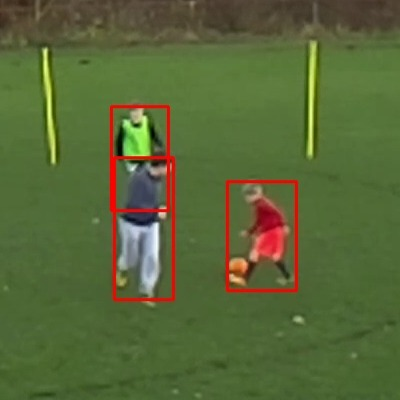
\includegraphics[scale=0.4]{D:/COMP30040/report/pic/3_new/on_seq_5.jpg} 
  \end{subfigure}
    \begin{subfigure}[b]{0.5\linewidth}
  \centering
	\includegraphics[scale=0.4]{D:/COMP30040/report/pic/3_new/off_seq_6.jpg} 
  \end{subfigure}
  \begin{subfigure}[b]{0.5\linewidth}
  \centering
	\includegraphics[scale=0.4]{D:/COMP30040/report/pic/3_new/on_seq_6.jpg} 
  \end{subfigure}
  \caption{时序检测结果比较(第二部分)。左侧:未使用先验知识;右侧:使用先验知识}
\end{figure}

\begin{figure}[h!]
  \begin{subfigure}[b]{0.5\linewidth}
  \centering
	\includegraphics[scale=0.4]{D:/COMP30040/report/pic/3_new/heu_false_off.jpg} 
  \end{subfigure}
  \begin{subfigure}[b]{0.5\linewidth}
  \centering
	\includegraphics[scale=0.4]{D:/COMP30040/report/pic/3_new/heu_false_on.jpg} 
  \end{subfigure}
  \caption{先验知识得到假阳。左侧:未使用先验知识;右侧:使用先验知识}
\end{figure}

\subsection{分类}
在从每帧中得到检测结果后,我使用分类器为每个检测到的运动员打标签。这一步打上的标签不会被直接用于追踪而是作为在标签校正中的基准信息。\\
考虑到样例清晰度低且为运动员打标签需要针对每个视频具体实现,我需要在给定的训练集上自己训练一个分类器。我建立分类器的思路参考了 [1]。首先我尝试使用其中推荐的超参数组合,即仅使用SIFT,k=11且词包大小为200,但这在我的系统中并未给出良好性能。因此我做了更多的实验,最终配置为使用基于MSER的SIFT,k=11且词包大小为200。
\subsection{追踪}
Tracking-by-detection 思想在该部分中被应用,意味着追踪是基于检测结果而非分类结果。理论上我们将对每个运动员建立一个追踪片段以储存检测结果序列,然而实际上对一段录播而言追踪片段的数量可能大于在视频中出现过的运动员的数量,因为运动员可能会多次进入或离开录像范围,且可能由于遮挡导致追踪丢失。如果强行建立与运动员数量相同的追踪片段,则某些片段可能由于运动员长时间离开录像范围而产生大量空白追踪,而将这些空白追踪全部放入片段不仅无意义还会占用大量内存空间。因此将追踪片数量段在系统中定死并不明智。\\
我实现追踪的方式基于 [2] 进行,运用了 Kalman滤波器进行预测及校正。[2] 中提到的一个问题是当遮挡出现时一个追踪片段可能会丢失对应运动员的定位,这是因为在足球运动中遮挡经常发生在进攻方试图绕过防守方时,而这经常包含复杂的移动技巧从而导致运动员改变方向。运动员的追踪基点在其实际检测由于遮挡而消失前也会由于检测框形状的变化而无规律运动,这为正确预测遮挡下的运动员位置更添难度,因此当预测位置向一个方向移动时,实际位置可能走向了另一方向,而这就导致了追踪丢失。\\
为了在一定程度上减轻该问题,我使用了略微复杂一些的预测模型。当实际检测与预测匹配时,一切和 [2] 中相同。当实际检测消失,只有预测位置可被使用时,我们使用一个变量$c$。$c$ 记录了从某运动员的实际检测最后一次出现后连续使用预测结果作为当前帧最终结果的帧数。当实际检测结果与预测结果匹配成功时,$c$恒为0; 当当前为仅使用预测结果的第一帧时,$c$=1; 当当前为第二帧时,$c$=2,以此类推。\\
$e^{-c}$ 被用于逐渐降低预测结果的移动速度以希望在实际检测再次出现时预测结果不会离其太远以至于超过了时序连贯中设定的阈值。因此在 Kalman 滤波器中最终的状态转移矩阵为:\\
\[\begin{bmatrix}1 & e^{-c}\frac{x_{k-1}-x_{k-2}}{y_{k-1}} \\e^{-c}\frac{y_{k-1}-y_{k-2}}{x_{k-1}} & 1 \end{bmatrix}\].\\
值得注意的是当运动员的实际检测被匹配时,c=0,$e^{-c}$=1,矩阵将与 [2] 中相同。
\subsection{追踪片段清理 \& 标签校正}
这里我们需要筛除显著错误的追踪片并为每个片段一个内部一致的标签。
\subsubsection{片段清理}
在检测阶段,多数假阳包含多于一个运动员(在遮挡出现时经常发生),但仍有少量假阳不含运动员。在多数时候它们会出现在某一帧中然后在下一帧消失,间隔长时间后再次出现(时间间隔远超过追踪中设定的连续使用预测值的最高次数)。根据前文中追踪的机制,在这种检测结果上会有新的追踪片段被建立,因为很有可能大多数运动员都更合适的检测结果进行匹配,未匹配的预测与该假阳结果间的距离也超过了时序连贯中设定的阈值。因此由此建立的追踪片段会只含有一个实际假阳检测,其长度比在运动员检测结果上上建立的追踪片段明显较短。可以简单设定一个长度阈值过滤掉这些追踪片段。
\subsubsection{Label correction}
这里我实现了最基础的标签校正。在第一次遍历目标录播后,追踪片段会包含运动员的轨迹信息,然而由于在追踪中采用 Tracking-by-detection,片段中的标签可能不完全相同。在这里我们将片段中出现最频繁的标签赋给整个片段。“多数决”中“多数只针对实际检测而言。在我的实现中,所有预测值的标签均采用实际检测消失前最后一个实际检测的标签,然而该标签仍旧可能是错误的,而之后所有预测值的标签则会有同样错误。因此预测值的标签不可被用于多数决。
\begin{figure}[h!]
  \begin{subfigure}[b]{\linewidth}
  \centering
    \includegraphics[scale=0.2]{D:/COMP30040/report/pic/3_new/no_occlusion.png} 
    \caption{普通情况下的成功}
  \end{subfigure}
  \begin{subfigure}[b]{\linewidth}
  \centering
    \includegraphics[scale=0.2]{D:/COMP30040/report/pic/3_new/success.png} 
    \caption{遮挡出现时的成功}
  \end{subfigure}
  \begin{subfigure}[b]{\linewidth}
  \centering
    \includegraphics[scale=0.2]{D:/COMP30040/report/pic/3_new/false_identity.png} 
    \caption{一个运动员被分配了错误的标签}
  \end{subfigure}
  \begin{subfigure}[b]{\linewidth}
  \centering
    \includegraphics[scale=0.2]{D:/COMP30040/report/pic/3_new/false_negative.png} 
    \caption{Tracking failure.}
  \end{subfigure}
  \caption{追踪失败}
  \begin{subfigure}[b]{\linewidth}
  \centering
    \includegraphics[scale=0.2]{D:/COMP30040/report/pic/3_new/occlu_fail.png} 
    \caption{遮挡导致的失败}
  \end{subfigure}
  \caption{最终结果示例}
\end{figure}

\subsection{显示}
之后我们便可以在目标录像中画出结果。在每个运动员上会画出三样东西:
\begin{itemize}
\item 1. 标出运动员位置的检测框,其颜色根据运动员标签决定;
\item 2. 在检测框上写出运动员身份标签,该身份决定了该运动员相关所有颜色;
\item 3. 代表运动员近期运动轨迹的曲线。
\end{itemize}
输出视频为\texttt{.mp4}格式以便复看。表明运动员身份与轨迹的追踪片段同样被作为中间结果输出,但可悲进一步利用。\\
\subsection{测试}
尽管我尝试的方法与 [1], [2] 中类似,但系统第一部分-检测已采用了不同方法,分类部分的超参数配置也发生了变化,因此对整个系统的评估需重新进行。相关工作在下一部分中陈述。
\newpage

\section{测评}
\subsection{检测}
\subsubsection{数据收集}
我对训练与测试视频进行了一些预处理以缩短数据收集时间。对于trainingVideo.mp4,收集从00:24,第二个运动员进入屏幕处开始;对于testingVideo.mp4, 从00:22,即第二个运动员出现处开始,在04:43,后续视频中不再有遮挡出现时结束。进行测评需要基准信息,我使用了同 [1] 中类似的方法收集,除了检测框从 Mask-RCNN 中得到。
\subsubsection{评价标准}
理想情况下,一个成功的检测应该(大致)包含一个运动员的整个身体;在实践中,那些在刚进入屏幕的运动员上得到的检测也该作数;同时,只含运动员身体的一部分或包含多个运动员的检测应被算作假阳。\\
检测质量在使用  提到的先验知识滤掉明显错误的假阳后再进行;或者说只在那些将要被进行分类并放入追踪片段的检测结果上进行,因为只有这部分结果才会对整个系统的表现产生影响。在一开始就被滤掉的检测对系统性能不会产生影响。\\
在 [1] 中,录播中运动员的数量在测试程序中被设为参数以估计运动员在所有帧中一共出现的次数,但我采用了更为精细的方法:\\
考虑到运动员有时会进入或离开屏幕范围,我首先估测了运动员数目保持恒定的各时间段。这可以通过每当在运动员进入或退出屏幕,即运动员数量变化时便暂停,并记录当前帧数,来达到近似精确的程度,这样在两次连续的记录之间应追踪的运动员数量保持恒定,而运动员在所有帧中出现的总次数可通过将每一段中运动员数量与该段帧长度相乘并将各段结果相加得到,这比仅用录播中多数时刻运动员出现的次数与帧长度相称得到结果更为准确。\\
我对一段视频中的检测结果进行了编程自动收集,并人工分辨了真阳和假阳,因为对一个检测结果是否包含正好一个运动员的整个身体(有时其部分身体被遮挡)的判断无法简单用脚本进行。\\
\subsubsection{测试与实验}
在下文中,运动员 A 着蓝色, B 着绿球衣, C 着红色, Scott 着黑色。\\
我手动在到处的检测结果中分辨了真阳与假阳并分别计数以给出精确率和召回率。\\
真阳:只含一个运动员的全部身体的检测结果。若该运动员的一部分被另一运动员的一部分遮挡但检测框仍紧贴该运动员外轮廓,或检测框在紧贴该运动员外轮廓时仍包括了另一运动员身体的一部分,是可以接受的。\\
\begin{figure}[h!]
\centering
  \begin{subfigure}[b]{0.15\linewidth}
  \centering
    \includegraphics[scale=0.4]{D:/COMP30040/report/pic/4/pos_1.jpg} 
    \caption{}
  \end{subfigure}
  \begin{subfigure}[b]{0.15\linewidth}
  \centering
    \includegraphics[scale=0.4]{D:/COMP30040/report/pic/4/pos_2.jpg} 
    \caption{}
  \end{subfigure}
  \begin{subfigure}[b]{0.15\linewidth}
  \centering
    \includegraphics[scale=0.4]{D:/COMP30040/report/pic/4/pos_3.jpg}
    \caption{} 
  \end{subfigure}
  \caption{真阳示例}
\end{figure}

\begin{figure}[h!]
\centering
  \begin{subfigure}[b]{0.25\linewidth}
  \centering
    \includegraphics[scale=0.4]{D:/COMP30040/report/pic/4/neg_1.jpg} 
    \caption{}
  \end{subfigure}
  \begin{subfigure}[b]{0.25\linewidth}
  \centering
    \includegraphics[scale=0.4]{D:/COMP30040/report/pic/4/neg_2.jpg} 
    \caption{}
  \end{subfigure}
  \begin{subfigure}[b]{0.25\linewidth}
  \centering
    \includegraphics[scale=0.4]{D:/COMP30040/report/pic/4/neg_3.jpg}
    \caption{} 
  \end{subfigure}
  \begin{subfigure}[b]{0.25\linewidth}
  \centering
    \includegraphics[scale=0.4]{D:/COMP30040/report/pic/4/neg_4.jpg} 
    \caption{}
  \end{subfigure}
  \begin{subfigure}[b]{0.25\linewidth}
  \centering
    \includegraphics[scale=0.4]{D:/COMP30040/report/pic/4/neg_5.jpg} 
    \caption{}
  \end{subfigure}
  \begin{subfigure}[b]{0.25\linewidth}
  \centering
    \includegraphics[scale=0.4]{D:/COMP30040/report/pic/4/neg_6.jpg} 
    \caption{}
  \end{subfigure}
  \caption{假阳示例}
\end{figure}
假阳:包含多个运动员完整轮廓的检测结果,对纯背景的检测或包含过多背景的结果。\\
图 给出了一些真阳示例。
\begin{itemize}
\item (b): 检测结果中运动员的部分身体被遮挡,但下边界可推断在其脚部附近。
\item (c): 检测框包含多个运动员,但其边界均紧贴统一运动员的身体轮廓。
\end{itemize}
当检测框包含一个运动员的部分身体,原因为其正在进入/离开屏幕时,该检测被算作真阳。\\
图 给出了一些假阳示例。
\begin{itemize}
\item (a): 检测框中包含一个运动员和其他物体。
\item (b),(c): 检测框包含多个运动员。 
\item (d): 检测框在运动员上/下方留白过多。
\item (e): 检测框内无人。
\item (f): 检测框只含多个运动员的部分身体。
\end{itemize}
当检测框包含一个运动员的部分身体,原因为其被遮挡幕时,该检测被算作假阳。\\
在我进行测试的两个视频中,我们基本可以知道每个运动员进入/离开屏幕的大致时间(鉴于这并不频繁),因此很容易可判断检测框队运动员的部分包括是由于何种原因,只需检查其出现时间即可。\\
在以上运动员出现总次数的计数标准下,裁剪过的 testingVideo.mp4/4peopleKickabout 25fps.mp4 中共有28795频次运动员出现次数,裁剪过的 trainingVideo.m4/4peopleKickabout2 30fps.mp4 中共有36319频次运动员出现次数。\\
在手动检查2视频的检测结果后,我发现运动员 C 的检测数量比其它人少(不通过严格计数便可得出结论)。这有两个原因:
\begin{itemize}
\item a. 遮挡频繁发生。C 在视频中显得更小,且由于低清晰度的关系,在 RPN 中对其的图像分割更为困难,尤其当C位于其他运动员后面时(某些情况下他会被完全遮挡)。
\item b. 由先验知识建立的阈值被用于筛掉那些尺寸过小而可能只含运动员身体一部分的检测框。但当 C 离屏幕过远时,其检测框尺寸也会落到阈值之下,这便导致了另一提升精确率还是召回率的两难问题。我的选择是提升精确率。
\end{itemize}
从表1实验结果中我们可以看到检测器有很高的精确率,但召回率较低,意味着该检测器强于使其给出的多数检测框正确,但在找到检测框方面能力较弱。几乎所有的检测失败均发生在部分或完全遮挡发生时,我们可从视频中看到在遮挡未发生时检测基本是连续的。\\
从表1-表5中我们可看到分割检测框的先验知识确实可帮助提升精确率与召回率。总体而言,更低的分割阈值可以给出更高的精确率与召回率。鉴于在遮挡未发生时该先验知识根本无法被用上,即此时检测结果不变,我们可以得出结论:该先验知识确实可以帮助减轻遮挡问题。\\
然而,这仍是一个十分原始的模型,并且只对两个运动员之间的遮挡适用。当遮挡在3个或以上数量运动员间发生时,该先验知识几乎不可能给出正确分割,因为他们的轨迹组合变得远更复杂。
\begin{table}[]
\centering
\begin{tabular}{|c|c|c|c|c|c|}
\hline
\multicolumn{3}{|c|}{trainingVideo} & \multicolumn{3}{c|}{testingVideo} \\ \hline
 & 真 & 假 &  & 真 & 假 \\ \hline
阳 & 24046 & 1140 & 阳 & 19721 & 1121 \\ \hline
阴 &  & 12273 & 阴 &  & 8179 \\ \hline
精确率 & \multicolumn{2}{c|}{93.25\%} & 精确率 & \multicolumn{2}{c|}{94.62\%} \\ \hline
召回率 & \multicolumn{2}{c|}{63.21\%} & 召回率 & \multicolumn{2}{c|}{68.49\%} \\ \hline
\end{tabular}
\caption{不使用先验知识时的混淆矩阵}
\end{table}

\begin{table}[]
\centering
\begin{tabular}{|c|c|c|c|c|c|}
\hline
\multicolumn{3}{|c|}{trainingVideo} & \multicolumn{3}{c|}{testingVideo} \\ \hline
 & 真 & 假 &  & 真 & 假 \\ \hline
阳 & 25042 & 848 & 阳 & 20583 & 794 \\ \hline
阴 &  & 11277 & 阴 &  & 8212 \\ \hline
精确率 & \multicolumn{2}{c|}{96.72\%} & 精确率 & \multicolumn{2}{c|}{96.29\%} \\ \hline
召回率 & \multicolumn{2}{c|}{68.95\%} & 召回率 & \multicolumn{2}{c|}{73.01\%} \\ \hline
\end{tabular}
\caption{阈值为1.2时的混淆矩阵}
\end{table}

\begin{table}[]
\centering
\begin{tabular}{|c|c|c|c|c|c|}
\hline
\multicolumn{3}{|c|}{trainingVideo} & \multicolumn{3}{c|}{testingVideo} \\ \hline
 & 真 & 假 &  & 真 & 假 \\ \hline
阳 & 24823 & 990 & 阳 & 20402 & 927 \\ \hline
阴 &  & 11496 & 阴 &  & 8393 \\ \hline
精确率 & \multicolumn{2}{c|}{96.16\%} & 精确率 & \multicolumn{2}{c|}{95.65\%} \\ \hline
召回率 & \multicolumn{2}{c|}{68.34\%} & 召回率 & \multicolumn{2}{c|}{72.36\%} \\ \hline
\end{tabular}
\caption{阈值为1.25时的混淆矩阵}
\end{table}

\begin{table}[]
\centering
\begin{tabular}{|c|c|c|c|c|c|}
\hline
\multicolumn{3}{|c|}{trainingVideo} & \multicolumn{3}{c|}{testingVideo} \\ \hline
 & 真 & 假 &  & 真 & 假 \\ \hline
阳 & 24987 & 778 & 阳 & 20421 & 956 \\ \hline
阴 &  & 11332 & 阴 &  & 7663 \\ \hline
精确率 & \multicolumn{2}{c|}{96.98\%} & 精确率 & \multicolumn{2}{c|}{95.53\%} \\ \hline
召回率 & \multicolumn{2}{c|}{68.80\%} & 召回率 & \multicolumn{2}{c|}{70.92\%} \\ \hline
\end{tabular}
\caption{阈值为1.3时的混淆矩阵}
\end{table}

\begin{table}[]
\centering
\begin{tabular}{|c|c|c|c|c|c|}
\hline
\multicolumn{3}{|c|}{trainingVideo} & \multicolumn{3}{c|}{testingVideo} \\ \hline
 & 真 & 假 &  & 真 & 假 \\ \hline
阳 & 24805 & 933 & 阳 & 20303 & 956 \\ \hline
阴 &  & 11514 & 阴 &  & 8492 \\ \hline
精确率 & \multicolumn{2}{c|}{96.37\%} & 精确率 & \multicolumn{2}{c|}{95.50\%} \\ \hline
召回率 & \multicolumn{2}{c|}{68.30\%} & 召回率 & \multicolumn{2}{c|}{70,50\%} \\ \hline
\end{tabular}
\caption{阈值为1.35时的混淆矩阵}
\end{table}
\subsection{分类}
我对分类的评估大致遵循了 [1] 中的想法,即测试不同的参数组合,调试超参数并给出混淆矩阵。然而在本部分中更为详细的结果将被给出以便分析。有时不同类别的精确率与召回率差距极大。鉴于我们的目标是尽可能增大每一类的精确率与召回率,仅给出各类相应值的平均值会将其中的过低值遮盖,从而并不合适。因此每一类的精确率与召回率将被给出,同时总体精度被附上以作参考。
\begin{table}[]
\centering
\begin{tabular}{|c|c|c|c|c|c|c|c|c|c|}
\hline
\multicolumn{1}{|l|}{by \%} & \multicolumn{4}{l|}{精确率} & \multicolumn{4}{l|}{召回率} & \multirow{2}{*}{精度} \\ \cline{1-9}
\multicolumn{1}{|l|}{筐数量} & A & B & C & scott & A & B & C & scott &  \\ \hline
16 & 89.47 & 9.30 & 34.18 & 87.90 & 1.96 & 2.54 & 99.69 & 69.34 & 43.38 \\ \hline
32 & 84.91 & 24.06 & 41.99 & 91.39 & 5.84 & 19.76 & 94.53 & 78.46 & 49.65 \\ \hline
64 & 72.13 & 22.58 & 42.33 & 91.40 & 8.46 & 22.38 & 87.92 & 74.46 & 48.31 \\ \hline
\end{tabular}
\caption{RGB 直方图, K=11}
\end{table}

\begin{table}[]
\begin{tabular}{|c|c|c|c|c|c|c|c|c|c|}
\hline
\multicolumn{1}{|l|}{by \%} & \multicolumn{4}{c|}{精确率} & \multicolumn{4}{c|}{召回率} & \multicolumn{1}{l|}{\multirow{2}{*}{精度}} \\ \cline{1-9}
BOW size & A & B & C & scott & A & B & C & scott & \multicolumn{1}{l|}{} \\ \hline
25 & 88.53 & 94.41 & 90.01 & 94.54 & 89.07 & 87.25 & 92.92 & 98.07 & 91.83 \\ \hline
50 & 94.69 & 93.97 & 89.56 & 96.23 & 89.92 & 91.83 & 94.07 & 98.42 & 93.56 \\ \hline
75 & 95.68 & 95.35 & 92.04 & 96.15 & 92.15 & 92.53 & 95.26 & 99.15 & 94.77 \\ \hline
100 & 94.47 & 94.87 & 93.25 & 96.05 & 92.11 & 94.11 & 94.11 & 98.34 & 94.67 \\ \hline
125 & 95.85 & 94.94 & 94.31 & 95.17 & 92.53 & 94.07 & 95.11 & 98.53 & 95.05 \\ \hline
150 & 96.79 & 94.69 & 93.93 & 95.13 & 91.73 & 94.88 & 95.38 & 98.46 & 95.11 \\ \hline
200 & 97.04 & 95.67 & 95.55 & 93.23 & 92.27 & 94.61 & 95.84 & 98.57 & 95.32 \\ \hline
\end{tabular}
\caption{MSER, K=11}
\end{table}

\begin{table}[]
\begin{tabular}{|c|c|c|c|c|c|c|c|c|c|}
\hline
\multicolumn{1}{|l|}{by \%} & \multicolumn{4}{c|}{精确率} & \multicolumn{4}{c|}{召回率} & \multicolumn{1}{l|}{\multirow{2}{*}{精度}} \\ \cline{1-9}
BOW size & A & B & C & scott & A & B & C & scott & \multicolumn{1}{l|}{} \\ \hline
25 & 77.24 & 74.65 & 71.22 & 92.46 & 64.5 & 62.42 & 95.30 & 91.61 & 78.46 \\ \hline
50 & 76.68 & 87.16 & 67.79 & 97.11 & 73.61 & 55.61 & 98.69 & 91.88 & 79.95 \\ \hline
63 & 80.75 & 87.95 & 63.75 & 97.36 & 69.38 & 56.19 & 98.96 & 92.46 & 79.25 \\ \hline
75 & 80.49 & 91.01 & 61.95 & 97.61 & 71.88 & 51.80 & 99.23 & 91.38 & 78.57 \\ \hline
87 & 84.34 & 93.08 & 59.25 & 98.87 & 70.65 & 52.30 & 99.34 & 91.31 & 78.41 \\ \hline
100 & 86.21 & 96.04 & 56.73 & 98.95 & 69.5 & 50.46 & 99.42 & 90.65 & 77.50 \\ \hline
125 & 85.78 & 95.44 & 52.04 & 99.36 & 61.03 & 45.15 & 99.5 & 89.76 & 73.86 \\ \hline
\end{tabular}
\caption{SIFT, K=11}
\end{table}

\begin{table}[]
\begin{tabular}{|c|c|c|c|c|c|c|c|c|c|}
\hline
\multicolumn{1}{|l|}{by \%} & \multicolumn{4}{c|}{精确率} & \multicolumn{4}{c|}{召回率} & \multicolumn{1}{l|}{\multirow{2}{*}{精度}} \\ \cline{1-9}
BOW size & A & B & C & scott & A & B & C & scott & \multicolumn{1}{l|}{} \\ \hline
25 & 91.60 & 84.59 & 86.90 & 96.89 & 82.30 & 84.5 & 96.5 & 96.15 & 89.86 \\ \hline
50 & 91.62 & 91.37 & 83.82 & 97.76 & 85.42 & 81.53 & 98.84 & 97.38 & 90.79 \\ \hline
75 & 90.30 & 94.27 & 83.76 & 98.96 & 87.80 & 79.11 & 99.19 & 99.38 & 91.37 \\ \hline
100 & 94.85 & 98.09 & 84.74 & 99.19 & 90.69 & 85.19 & 99.38 & 99.46 & 93.68 \\ \hline
150 & 96.41 & 98.46 & 80.32 & 99.38 & 85.76 & 86.19 & 99.53 & 98.96 & 92.61 \\ \hline
150 & 97.95 & 99.22 & 78.18 & 99.26 & 86.38 & 84.07 & 99.53 & 99.03 & 92.25 \\ \hline
\end{tabular}
\caption{SIFT+MSER, K=11}
\end{table}

\begin{table}[]
\begin{tabular}{|c|c|c|c|c|c|c|c|c|c|}
\hline
\multicolumn{1}{|l|}{by \%} & \multicolumn{4}{c|}{精确率} & \multicolumn{4}{c|}{召回率} & \multicolumn{1}{l|}{\multirow{2}{*}{精度}} \\ \cline{1-9}
\begin{tabular}[c]{@{}c@{}}Feature \\ combined\end{tabular} & A & B & C & scott & A & B & C & scott & \multicolumn{1}{l|}{} \\ \hline
SIFT & 72.13 & 22.59 & 42.34 & 91.40 & 8.46 & 22.38 & 87.96 & 74.46 & 48.31 \\ \hline
MSER & 72.13 & 22.59 & 42.34 & 91.40 & 8.46 & 22.38 & 87.96 & 74.46 & 48.31 \\ \hline
SIFT+MSER & 72.13 & 22.59 & 42.34 & 91.40 & 8.46 & 22.38 & 87.96 & 74.46 & 48.31 \\ \hline
\end{tabular}
\caption{混合使用特征, K=11, RGB 筐数量=64, 词包大小=150}
\end{table}

\begin{table}[]
\begin{tabular}{|c|c|c|c|c|c|c|c|c|c|}
\hline
\multicolumn{1}{|l|}{by \%} & \multicolumn{4}{c|}{精确率} & \multicolumn{4}{c|}{召回率} & \multicolumn{1}{l|}{\multirow{2}{*}{精度}} \\ \cline{1-9}
K & A & B & C & scott & A & B & C & scott & \multicolumn{1}{l|}{} \\ \hline
5 & 96.37 & 95.28 & 94.15 & 94.94 & 91.96 & 94.95 & 95.42 & 98.34 & 95.17 \\ \hline
11 & 97.04 & 95.67 & 95.55 & 93.23 & 92.26 & 94.61 & 95.84 & 98.57 & 95.32 \\ \hline
21 & 97.26 & 95.91 & 96.15 & 90.92 & 91.53 & 93.91 & 95.19 & 99.07 & 94.93 \\ \hline
41 & 94.85 & 98.09 & 84.74 & 99.19 & 90.69 & 85.19 & 99.38 & 99.46 & 93.68 \\ \hline
81 & 97.86 & 96.28 & 97.25 & 85.16 & 88.11 & 92.76 & 93.99 & 99.61 & 93.62 \\ \hline
161 & 98.57 & 96.56 & 97.66 & 80.01 & 85.07 & 91.83 & 91.68 & 99.76 & 92.09 \\ \hline
\end{tabular}
\caption{MSER,词包大小=200}
\end{table}

表 给出了对 K 值,词包大小及特征组合的调参结果。\\
一个格外显眼的结果是表10中结果完全相同,且这三个结果也与表6的最后一行基本相同,差距只有0.05\%。这是因为 RGB 直方图对聚类的影响过强导致其它特征相比之下基本等同于噪声。
我们可以看到加入 RGB 直方图的特征组合在所有组合中表现最差,且增加筐数量基本没用。这显示了 RGB 直方图在该任务中的灾难性后果并表明特征向量在空间中基本无法区分。鉴于使用的训练样例中不包含遮挡,其原因可能有两种:
\begin{itemize}
\item 1. 样例清晰度过低,同时运动员动作变化极大,导致同一运动员的不同样例直方图变化过大;
\item 2. 样例背景不同。某些样例的背景包含黄色或橙色的杆子,有些包含了足球,还有些只有纯背景,为直方图增加了额外变数。
\end{itemize}
在得到这些结果后,我们可以大致看到特征组合的选择才能显著影响分类结果。在所有组合中单用MSER能达到最好效果,SIFT 与 MSER 混用效果略微下降,单用SIFT表现最差。调整词包大小有一定作用,但比起对特征组合的选择而言效果有限,在我的上述实验中最大提升为5\%.\\
表11给出了对K值的实验结果。我们可看到在 K=11 时精度达到最大值。鉴于在该表中精确率与召回率均高而均衡,因此对每一类的结果单独关注不再必要。
\newpage

\section{反思}
总体而言该项目是成功的。在该系统中,运动员能以令人满意的精度被检测、分类并追踪。
\subsection{成功}
该项目的最终目标是在系统中根据运动员的标签及轨迹自动生成战术。然而在当前的完成版本中下列任务已被达成:\\
它利用了深度学习进行运动员检测,达到68.95\% \& 73.01\%的召回率与96.72\% \& 96.29\%的精确率。仅通过比较进行运动员检测后在录像中画出的结果,我们便可发现它确实较使用背景消除与基于 HOG 的 SVM 有所提升。检测失败基本在严重遮挡出现时发生,而轻度遮挡可被妥善处理。在遮挡未发生时,对运动员的检测基本是连续的。\\
在运动员分类上的精度进一步被提高,平均精确率为95.37\%,平均召回率为95.32\%。鉴于所给样例的分辨率之低,这样的准确率已经相当之高,我们可以说在分类阶段基本不会产生严重问题。\\
在追踪中用了 Tracking-by-detection 思想并使用时序连贯规范预测结果与检测结果间的匹配,Kalman 滤波器被用于调整检测结果并给出预测,这在检测失败时尤为重要。
\subsection{提升}
在该项目中,更多的提升与试验可被完成。\\
目前使用的泛用检测器可以给出令人满意的结果,但运行时间过长,大致2-4秒才能处理一帧。鉴于当前使用的网络中只有检测功能被使用,这里的模型可替换为更为轻量的版本,例如 Faster-RCNN。这将显著减少在视频中的处理时间。在处理遮挡问题上,一种可能的方法是增加对应该情况的正样本以增强模型的应对能力,另一方法是增加摄像机数目以从一开始便回避该问题。
基于 MSER 的 SIFT 已被证明在运动员分类低清人像上十分管用,但还可作进一步提升。鉴于神经网络在分类任务上被证明十分成功且强于特征提取,它也可被用于该任务中。\\
目前在 Kalman 滤波器中预测基点为检测框的中心,但有时其会随着检测框的变化而发生不规则移动,且这在运动员基本成直线运动时仍在发生。该问题会为预测带来问题,且如果遮挡同时发生则遮挡消失后追踪结果很可能丢失目标。因此需要既能表示运动员位置又可对检测框形状变化免疫的追踪基点被提出。本项目中采用了略微更复杂的预测模型,但效果并不明显。之后需要尝试更多的预测模型。\\
在该项目中出现了一个和追踪相关的问题:在运动员过于接近时,对一个运动员的检测会被赋给另一个运动员,且从该时刻开始两个追踪片段交换了追踪对象。其在标签校正阶段造成的问题是在上述两个追踪片段中前一段与后一段的检测不是属于同一运动员的。理论上一个追踪片段中的标签应该全部相同,因此在最后将追踪片段画到视频中时这两个追踪片段在部分时间内会将属于本运动员的检测框/轨迹与标签画在另一运动员上。可能的解决方法是更改将检测框赋给追踪片段的方法,更改检测方式或者借助其它知识在标签校正前将相关追踪片段从出问题的地方切开并拼接到另一片段上。\\
目前在标签校正中值采用了最基本的方法,其问题在于有些时候给出追踪片段的标签是相同的。该问题可能通过如 [3] 中使用加入同一时刻的追踪片段间互斥关系的完整版本的条件随机场解决,而非向 [2] 中的简化版本一样不加入互斥关系。
\subsection{未来工作}
达到该课题最终目标仍有距离,为了取得进展还有更多工作可被完成:\\
遮挡始终是主要问题并且阻碍了总体性能的提升。增加摄像机可能是一种方法,我们还可以尝试将运动员的位置映射到虚拟球场上,这会使得追踪更加精确,轨迹更容易预测,同时避免了运动员人像尺度变化问题。\\更多的特征可被尝试用于分类,同时可以借助神经网络的力量。
更先进的方式可被用于进行标签校正,其中一种是像 [3] 中一样利用条件随机场。在收集到运动员的轨迹和身份信息之后,我们可以进行例如运动员移动总距离的基本信息统计。我们也可以为运动员的位置关系赋予意义,例如判断运动员是否越位。额外追踪足球的位置可能会给我们更多有用的信息,例如持球者和周围运动员采取的策略,但这需要更为复杂的检测与分类模型。
\subsection{结论}
该课题的目标是研发一个可以在低清体育录播中自动识别与追踪运动员的系统,远期目标为根据轨迹与身份信息自动生成运动员表现并分析采用的策略。我为该系统的四部分(检测,分类,追踪,标签校正)分别实现一系列python脚本:基于模型的检测器被用于检测,从 MSER 中 提取的 SIFT 特征被使用KNN用于分类;Kalman 滤波器与 Tracking-by-detection 思想被用于追踪。给定一段从静止相机产出的录播,系统输出是一段附上运动员检测框,标签及轨迹信息的视频,且每个运动员用对应颜色表示身份。通过进行大量实验,我对检测与分类部分的超参数进行了调参并给出了不同标准的评估结果。在检测中,精确率约为96\%,召回率约为70\%;分类中检测率与召回率均达到95\%。
\newpage

\begin{thebibliography}{2}
\bibitem{1} A. Dunlop. Tracking Football Players, 2017.
\bibitem{2} S. Akerman. Tracking Football Players, 2018.
\bibitem{3} W. L. Lu, J. A. Ting, K. P. Murphy, and J. J. Little. Identifying players in broadcast sports videos using conditional random fields. In \textit{CVPR 2011}, pages 3249–3256, June 2011.
\bibitem{4} Michael Beetz, Suat Gedikli, Jan Bandouch, Bernhard Kirchlechner, Nico von
Hoyningen-Huene, and Alexander Cli↵ord Perzylo. Visually tracking football games
based on tv broadcasts. In \textit{IJCAI}, pages 2066–2071, 2007.
\bibitem{5} Jia Liu, Xiaofeng Tong, Wenlong Li, Tao Wang, Yimin Zhang, and Hongqi Wang.
Automatic player detection, labeling and tracking in broadcast soccer video. \textit{Pattern Recogn. Lett.}, 30(2):103–113, January 2009.
\bibitem{6} K. He, G. Gkioxari, P. Dollár and R. Girshick, "Mask R-CNN," \textit{2017 IEEE International Conference on Computer Vision (ICCV), Venice}, 2017, pp. 2980-2988.
\bibitem{7} M Manafifard, H Ebadi, and H Abrishami Moghaddam. A survey on player tracking in soccer videos. \textit{Computer Vision and Image Understanding}, 2017.
\bibitem{8} Nir Friedman and Stuart Russell. Image Segmentation in Video Sequences: A Probabilistic Approach. In \textit{Proceedings of the Thirteenth Conference on Uncertainty in Artificial Intelligence}, UAI’97, pages 175–181, San Francisco, CA, USA, 1997. Morgan Kaufmann Publishers Inc.
\bibitem{9} Navneet Dalal and Bill Triggs. Histograms of Oriented Gradients for Human Detection. In \textit{Computer Vision and Pattern Recognition, 2005. CVPR 2005. IEEE Computer Society Conference} on, volume 1, pages 886–893. IEEE, 2005.
\bibitem{10} R. Girshick, J. Donahue, T. Darrell and J. Malik, "Rich Feature Hierarchies for Accurate Object Detection and Semantic Segmentation," \textit{2014 IEEE Conference on Computer Vision and Pattern Recognition}, Columbus, OH, 2014, pp. 580-587.
\bibitem{11} David G. Lowe. Object recognition from local scale-invariant features. In \textit{Proceedings of the International Conference on Computer Vision-Volume 2 - Volume 2,} ICCV ’99, pages 1150–, Washington, DC, USA, 1999. IEEE Computer Society.
\bibitem{12} R. E. Kalman. A new approach to linear filtering and prediction problems.
\textit{Transactions of the ASME - Journal of Basic Engineering}, 82:35–45, 1960.
\bibitem{13} OpenCV Library and Documentation. OpenCV HOG detector. \url{https://docs.opencv.org/3.4.2/d1/dc5/tutorial_background_subtraction.html}. [Online: accessed May 1, 2020].
\bibitem{14} OpenCV Library and Documentation. Opencv findcontours function. \url{https://docs.opencv.org/3.4.2/d4/d73/tutorial_py_contours_begin.html}. [Online; accessed May 1, 2020].
\bibitem{15} OpenCV Library and Documentation. OpenCV HOG detector.
\url{https://docs.opencv.org/3.4.2/d5/d33/structcv_1_
1HOGDescriptor.html#details}. [Online: accessed May 1, 2020].
\bibitem{16} OpenCV Library and Documentation. OpenCV HOG descriptor.
\url{https://docs.opencv.org/3.4.2/d5/d33/structcv_1_
1HOGDescriptor.html#details. https://docs.opencv.org/3.4.2/d5/d33/structcv_1_1HOGDescriptor.html#a723b95b709cfd3f95cf9e616de988fc8}. [Online: accessed May 1, 2020].
\bibitem{17} OpenCV Library and Documentation. OpenCV SVM Classifier. \url{https://docs.opencv.org/3.4.2/d1/d73/tutorial_introduction_to_svm.html}. [Online: accessed May 1, 2020].
\bibitem{18} Waleed Abdulla. (2017). Mask R-CNN for object detection and instance segmentation on Keras and TensorFlow. \url{https://github.com/matterport/Mask_RCNN}.
\bibitem{19} Tsung-Yi Lin, Michael Maire, Serge Belongie, Lubomir Bourdev, Ross Girshick, James Hays, Pietro Perona, Deva Ramanan, C. Lawrence Zitnick, \& Piotr Dollár. (2014). Microsoft COCO: Common Objects in Context.
\end{thebibliography}


\end{document}
